\PassOptionsToPackage{hyphens}{url}
\documentclass[preprint,12pt,nopreprintline]{elsarticle}
\usepackage{graphicx}    % in your preamble
%% Use the option review to obtain double line spacing
%% \documentclass[authoryear,preprint,review,12pt]{elsarticle}

%% Use the options 1p,twocolumn; 3p; 3p,twocolumn; 5p; or 5p,twocolumn
%% for a journal layout:
%% \documentclass[final,1p,times]{elsarticle}
%% \documentclass[final,1p,times,twocolumn]{elsarticle}
%% \documentclass[final,3p,times]{elsarticle}
%% \documentclass[final,3p,times,twocolumn]{elsarticle}
%% \documentclass[final,5p,times]{elsarticle}
%% \documentclass[final,5p,times,twocolumn]{elsarticle}

\usepackage{hyperref}           % clickable links
\usepackage{breakurl}           % breaks URLs in bibliography (with latex)
\usepackage{etoolbox}           % allows patching of commands
\usepackage{booktabs}

\hypersetup{
    hidelinks,
    breaklinks=true
}

\def\UrlBreaks{\do\/\do-\do.\do:\do_}

\usepackage{amssymb}
\usepackage{float}
\usepackage{eurosym}
%% The amsmath package provides various useful equation environments.
\usepackage{amsmath}
%% The amsthm package provides extended theorem environments
%% \usepackage{amsthm}

%% The lineno package adds line numbers. Start line numbering with
%% \begin{linenumbers}, end it with \end{linenumbers}. Or switch it on
%% for the whole article with \linenumbers.
%% \usepackage{lineno}

\begin{document}

\begin{frontmatter}

%% Title, authors and addresses

%% use the tnoteref command within \title for footnotes;
%% use the tnotetext command for the associated footnote;
%% use the fnref command within \author or \affiliation for footnotes;
%% use the fntext command for the associated footnote;
%% use the corref command within \author for corresponding author footnotes;
%% use the cortext command for the associated footnote;
%% use the ead command for the email address,
%% and the form \ead[url] for the home page:
%% \title{Title\tnoteref{label1}}
%% \tnotetext[label1]{}
%% \author{Name\corref{cor1}\fnref{label2}}
%% \ead{email address}
%% \ead[url]{home page}
%% \fntext[label2]{}
%% \cortext[cor1]{}
%% \affiliation{organization={},
%%             addressline={},
%%             city={},
%%             postcode={},
%%             state={},
%%             country={}}
%% \fntext[label3]{}

\title{Integrating societal preferences: Decentralization of the European energy network}
%% use optional labels to link authors explicitly to addresses:
%% \author[label1,label2]{}
%% \affiliation[label1]{organization={},
%%             addressline={},
%%             city={},
%%             postcode={},
%%             state={},
%%             country={}}
%%
%% \affiliation[label2]{organization={},
%%             addressline={},
%%             city={},
%%             postcode={},
%%             state={},
%%             country={}}

\author{Kristoffer Hedegaard Aden\\Aarhus University\\Student ID: 201905079} %% Author name
%% Abstract
\begin{abstract}
%% Text of abstract
Filler
\end{abstract}

%% Keywords
\begin{keyword}

European energy system \sep De-centralization \sep De-carbonization \sep PyPSA-EUR \sep Energy systems modeling \sep Fairness in energy transitions


%% keywords here, in the form: keyword \sep keyword

%% PACS codes here, in the form: \PACS code \sep code

%% MSC codes here, in the form: \MSC code \sep code
%% or \MSC[2008] code \sep code (2000 is the default)

\end{keyword}

\end{frontmatter}

%% Add \usepackage{lineno} before \begin{document} and uncomment 
%% following line to enable line numbers
%% \linenumbers

%% main text
%%

\newpage

\section{Introduction}
In a world where the necessity of reducing the carbon emissions of our energy networks is no longer a question but a requirement careful and deliberate planning of the energy system of our future is needed. When the Paris Climate agreement was signed into action in 2015 it signaled the commitment of the United Nations to reducing their overall carbon footprint \cite{ParisAgreementUNFCCC}. This common goal and understanding of the necessity of decarbonization was a crucial step towards a more sustainable world, and providing a common base understanding of what needs to be done, but also provides a massively complicated technological challenge that must be solved in order for the agreement to be fulfilled.

\medskip
\noindent Somewhat unique to the issue of decarbonization in the European Union, is the fact that, although the Paris Climate Agreement signifies the common goal of decarbonization, The Union is still comprised of many different countries with many different political ideologies, laws, societal preferences and goals of their own. This means that although it has long been known that a shared and interconnected energy grid is the most efficient and economically preferable solution, as seen for example in \cite{rodriguezCostoptimalDesignSimplified2015a}, reality becomes a lot more complicated as the member nations also must have their own best interest in mind.

\medskip
\noindent Historically the impact of the union being made up of self-centered actors has often been discarded when trying to construct the electricity grid of the future, if for no other reason than the fact that implementing social preferences and societal paradigms in strict mathematical models of the European energy system is a challenging problem \cite{pfenningerEnergySystemsModeling2014}. These models that typically aim to reduce the overall cost of the system as the primary objective are often meant to be used used as the basis for developing the future energy network and legislation. However using this least-cost optimization approach without considering social paradigms in the European Union tends to produce system models that, although being economically efficient at achieving decarbonization targets, that are intrinsically tied to the assumption that the EU has complete control over the member nations individual energy grids.

\medskip
\noindent This approach of reducing the optimization problems to purely techno-economic problems that prioritize cost reduction over feasibility has helped achieve significant insights into decarbonization strategies for the European Union \cite{henkeComparingEnergySystem2024}, but tends to lead to the energy system becoming heavily centralized \cite{eriksenOptimalHeterogeneitySimplified2017a}. Centralization in the context of energy systems refer to the majority of resources being pooled into a few areas that are favorable to the system in some way, be that installing a lot of wind turbines in a region with a lot of wind, maintaining energy production in regions close to where the energy is needed or any number of other mechanisms that result in a proportionally large investment into infrastructure in a single region. While centralization as a strategy is often the most cost efficient strategy it leads to a suite of other challenges.

\medskip
\noindent Two such challenges are those of physical security and and political feasibility. With the recent surge in so-called hybrid attacks on European energy infrastructure\cite{ScaleRussianSabotage}, the focus on physical security has increased. If a system is overly centralized it means that a large amount of critical infrastructure is installed on a relatively small area. This makes the infrastructure an obvious target for such hybrid attacks as a single hostile action can impact more infrastructure and more people. As for the political feasibility, nations who end up as net energy importers become less self sufficient and increasingly reliant on the net exporting regions. This shift in power-balance heavily favors the net exporters and as such may face resistance from net importing nations that wish to remain at a high degree of self sufficiency.    

\medskip
\noindent The objective of this masters thesis is to incorporate societal paradigms and priorities in the form of decentralization into a macro-scale energy network model of the EU, and to analyze and expose the mechanisms behind de-carbonization and its interactions with decentralization. The main hypothesis is that, by incorporating decentralization, the resulting networks will illuminate alternative transition pathways. This in tun may then help develop a workflow that by incorporating societal paradigms and reviewing their system impacts, will help close the gap between the models used to inform energy policy makers and the results of the proposed policies. Although this workflow and methodology may in time prove relevant for policy makers to understand, the target audience of this master's thesis remains peers in the field of energy system modeling who may draw inspiration from the intersection between societal paradigms and strict mathematic modeling that this work represents. It is also for this reason that all the data and code used to produce the results which can be seen in this paper is openly available in a public repository under an open science license\cite{GNUGeneralPublic}.

\section{Nomenclature}

\begin{tabular}{ll}
\textbf{Table Example} & \\
\hline
C1 R1 & C1 R2 \\
C2 R1 & C2 R2 \\
\end{tabular}

\section{Methodology}
Many energy modeling frameworks and pieces of commercially available software for optimizing nodal-networks exist. The work represented by this paper utilizes the open-source framework PyPSA (Python for power system analysis \cite{PyPSA}). The reasoning for this is twofold: Firstly PyPSA is completely free and open source to use. This encourages open and collaborative science as well as transparency in the philosophy behind the energy system modeling. Secondly PyPSA consists of two separate parts. A modeling workflow based in the Python programming language, and a large database containing relevant open source data for constructing models, particularly of the European Union. This dataset is referred to as PyPSA-Eur\cite{PyPSAEur} and is invaluable in its quality of data for building macro energy system models in the PyPSA workflow. This masters thesis utilizes both parts of the PyPSA environment. Acting as a baseline for all of the network topology for the European Union is a pre-compiled network developed with PyPSA-EUR using the default settings as published in the Zenodo repository \cite{horschPyPSAEurOpenOptimisation2023}.

\medskip
\noindent The simple philosophy behind the PyPSA models is that a network is perceived as multiple interconnected nodes. These nodes and connections are then given a set of constraints that define the feasible solution space. Examples of constraints could be that each node is assigned an electrical load that must be serviced based on historical consumption, capacity factor time-series based on solar- and wind-patterns, or maximum or minimum capacity constraints like a maximum allowable power flow from one node to another representing the transmission infrastructure in the network. The network used in this master's thesis is a 37 node network representing the 25 (excluding the island states of Malta and Cyprus) member nations of the EU. Additionally Switzerland, Norway, Bosnia-Herzegovina, Albania, Montenegro, North Macedonia, The United Kingdom and Serbia are included as their electrical infrastructure is connected to that of the EU. The following nations are also represented by more than one node as they have large populations on islands: Denmark, Spain, Great Britain and Italy.

\medskip
\noindent These nodes are then interconnected with HVDC and AC links and lines respectively. The nodes are then each assigned load patterns, and 

\subsection{Optimization strategy}
Optimizing complex energy networks with many variables and constraints is computationally very intensive. For this reason the optimizations performed for this master's thesis have exclusively been performed on a High Performance Computing (HPC) environment. More specifically the UCloud HPC operated by SDU \cite{UCloudUserGuide}. The optimizations were typically run on a set of 4 machines, each with an Intel Xeon Gold 6130 CPU and took on average 12 core-hours apiece to achieve an optimal solution. The optimization algorithm was chosen as the Barrier method in the commercial optimizer by Gurobi, chosen primarily for its numerical stability \cite{BarrierLoggingGurobi}.

\subsubsection{Objective functions and constraints}
Objective functions in  PyPSA and interacting with Gurobi. Adding the de-carbonization constraint to the least cost system

\medskip
\noindent In order to optimize the network first an objective function must be defined. An objective function is, as the name suggests, the function which when minimized or maximized leads to the objective of the optimization to be achieved. The objective function for finding the cheapest possible electrical system is defined as minimizing the sum of all the costs:

\medskip
\noindent Equation:

\begin{equation}
  \scalebox{0.8}{$
    \begin{aligned}
      \min\,&\Bigl(\sum_{n}\text{generation costs}
                 + \text{storage costs}
                 + \text{transmission costs}
             +\sum_{n,t}\text{variable costs}\Bigr)
    \end{aligned}
  $}
  \label{eq:cost_min}
\end{equation}
\medskip
\noindent Here $n$ denotes the set of all nodes, and $t$ denotes the set of all snapshots during the timeframe. However in order to construct a feasible solution space the objective function must be defined by a set of bounding constraints. Initially an equality constraint is defined so that, for each snapshot, all nodes must have their electricity demand met by a combination of energy production and nodal balancing:

\begin{equation}
\text{generation}_{n,t} + \text{balance}_{n,t}
= \text{demand}_{n,t}
\quad\longleftrightarrow\quad
\lambda_{n,t}
\quad\forall\,n,t
\label{eq:load_balance}
\end{equation}



\subsection{Least-cost system}
Introduction to least-cost systems and their purpose as a baseline.
\subsubsection{Modeling}
Modeling assumptions and methodology. Describing network topology and cost modeling.
\subsection{Decentralized systems}
Introduction to the secondary decentralizing sweeps
\subsubsection{Measures of decentralization}
Discussion on Standard deviation approach vs Gini Approach
\subsubsection{Linear systems}
Talking points on avoiding non-convex solution spaces
\subsubsection{Added constraints}
Discussing the K-constrains introduced for decentralization
\subsubsection{Avoiding constraint interactions}
Talking about how the normal K approach does not work as it leads to over de-carbonization
\section{Results}
Introduction to results
\subsection{Least-cost systems}
Maps and figures showing a few least-cost networks, their optimized topology and key figures like system cost and marginal prices.

\medskip
\noindent

\newpage
\subsection{Zero cost condition, brownfield systems and scarcity-rents}
\noindent
When reviewing the electricity prices associated with the optimized networks, it is of interest to compare two different cost measures: The mean marginal demand-weighted price and the levelized cost of electricity (LCOE). The mean marginal demand-weighted price is defined as:

\begin{equation}
\text{Mean Marginal Demand-Weighted Price}
=
\frac{\sum_{t \in T} \sum_{n} \left( L_{n,t} \times \lambda_t \right)}
{\sum_{t \in T} \sum_{n} L_{n,t}}
\end{equation}

\noindent
For time \textit{t}, Nodes \textit{n}, Loads \textit{L} and marginal price \textit{$\lambda$}. This cost measure represents the average price that consumers pay for electricity over the entire time period, weighted by their demand. The other cost measure, the levelized cost of electricity (LCOE) is defined as:
\begin{equation}
\text{LCOE}
=
\frac{\sum_{t \in T} \sum_{g}
\left( \text{Capital Costs}_{g,t} + \text{Marginal Costs}_{g,t} \right)}
{\sum_{t \in T} \sum_{n} L_{n,t}}
\end{equation}


\noindent
For generator technologies \textit{g}. LCOE represents the average cost of producing electricity over the lifetime of the system.

\medskip
\noindent
Seen below in Figure \ref{fig1} is a plot comparing the mean levelized cost of electricity for the different levels of decarbonization, compared to the mean marginal demand-weighted price:

\begin{figure}[H]
\centering
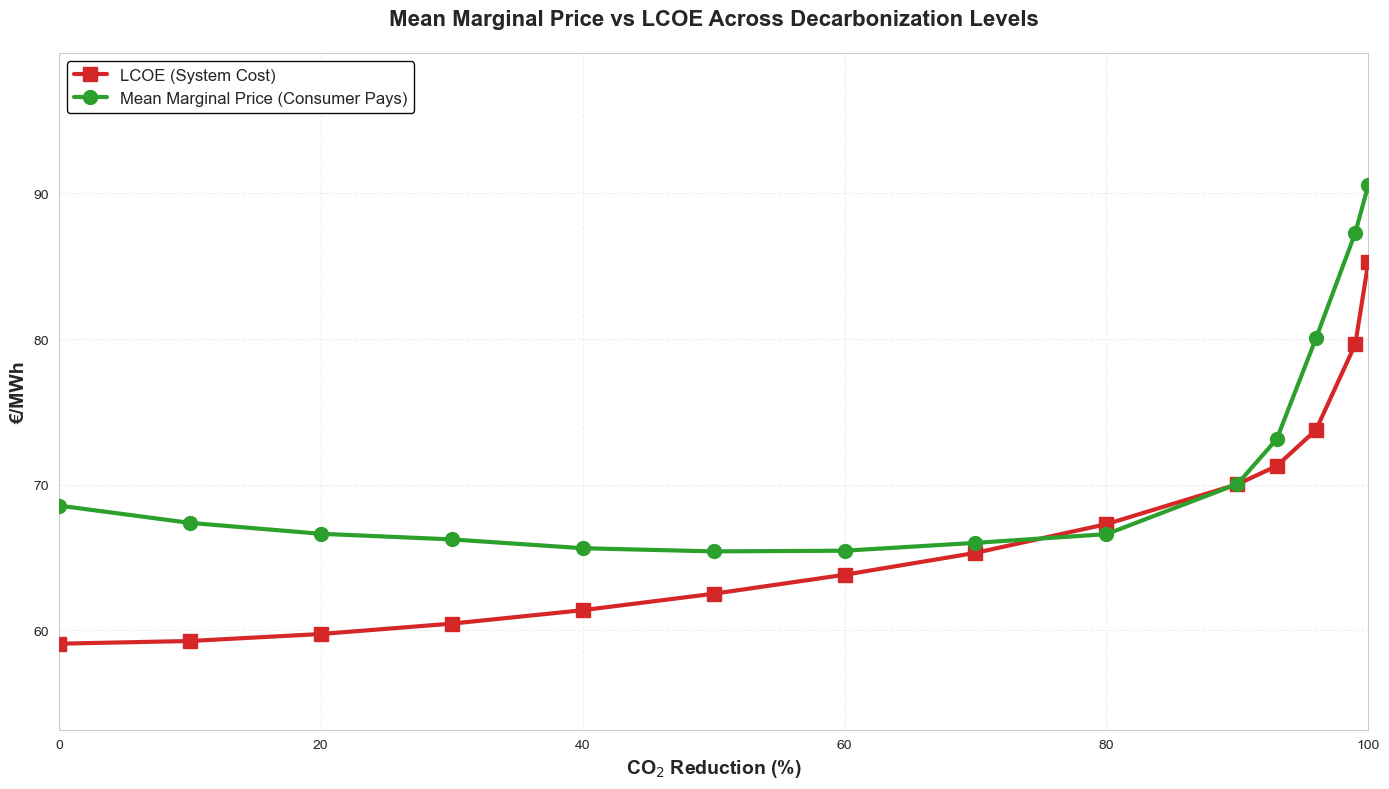
\includegraphics[width=\linewidth]{doc/Margnal_vs_LCOE_temp.png}
\caption{Comparison of mean LCOE and mean marginal price}
\label{fig1}
\end{figure}


\medskip
\noindent
This plot shows two different interesting results. Firstly it can be seen that as the system begins to decarbonize, initially the mean marginal demand weighted price \textit{decreases} before increasing dramatically at high levels of decarbonization.
Secondly it can be seen that for a majority of decarbonization levels a significant gap between the two cost measures is present.

\medskip
\noindent
Traditionally optimized energy system models such as the ones produced by PyPSA must adhere to the zero-profit condition \cite{kies_noprofit_pypsa}:

\begin{equation}
\sum_{t \in T} \sum_{n} \left( L_{n,t} \times \lambda_t \right)
=
\sum_{t \in T} \sum_{g}
\left( \text{Capital Costs}_{g,t} + \text{Marginal Costs}_{g,t} \right)
\end{equation}

\noindent
This equation states that for all times the demand-weighted marginal price in all nodes must be equal to the sum of the capital and marginal costs across all technologies and times. Or, in other words: The revenue must be equal to the expenditure.
However, critically, the zero-profit condition applies to long-run competitive equilibrium subject to the following assumptions:
\begin{itemize}
  \item All capacity is free to expand and contract in order to achieve optimality.
  \item No artificially imposed constraints on the system.
  \item Steady state market conditions.
\end{itemize}

\medskip
\noindent
This clashes with the modelling methodology in several ways. The optimized model is a \textit{Brownfield} system, meaning that even before optimization some fossil generation capacity exists in the system. As stated in the modelling section XXX, fossil generation capacity is allowed to contract but not to expand as constrained by:
\begin{equation}
  p_{\text{nom}} \leq p_{\text{nom, max}} = p_{\text{nom, baseline}}
\end{equation}

\noindent
This means that the zero profit condition does not apply to optimization performed in this thesis, which leads to the difference between levelized cost and mean marginal price, also known as scarcity rent, as seen in Figure \ref{fig1}. The scarcity rents manifest when the optimizer ideally would increase capacity to meet demand, but is constrained by a binding capacity constraint.

\medskip
\noindent
Imagine for example that a fossil fuel-based generator is producing electricity at a lower marginal cost than the current market price. If the fossil based generator was allowed to expand, this would naturally attract additional fossil based generation to the market, until it becomes saturated and the mean marginal demand weighted price decreases to the point where the fossil generator is no longer profitable. However, as the fossil generator is not allowed to expand capacity, it can continue to produce electricity at a profit, leading to the scarcity rents seen in the system. This is the primary driving mechanism behind the gap between LCOE and mean marginal demand weighted prices seen in Figure \ref{fig1}.

\medskip
\noindent
This mechanism also applies to non-extendable renewable generation capacity, like nuclear, geothermal and biomass, as well as non-extendable storage like pumped hydro-storage.
Pictured below, in Figure \ref{fig2} is the evolution of the contribution to the total scarcity rent from the different technologies not constrained by the zero-profit condition:

\begin{figure}[H]
\centering
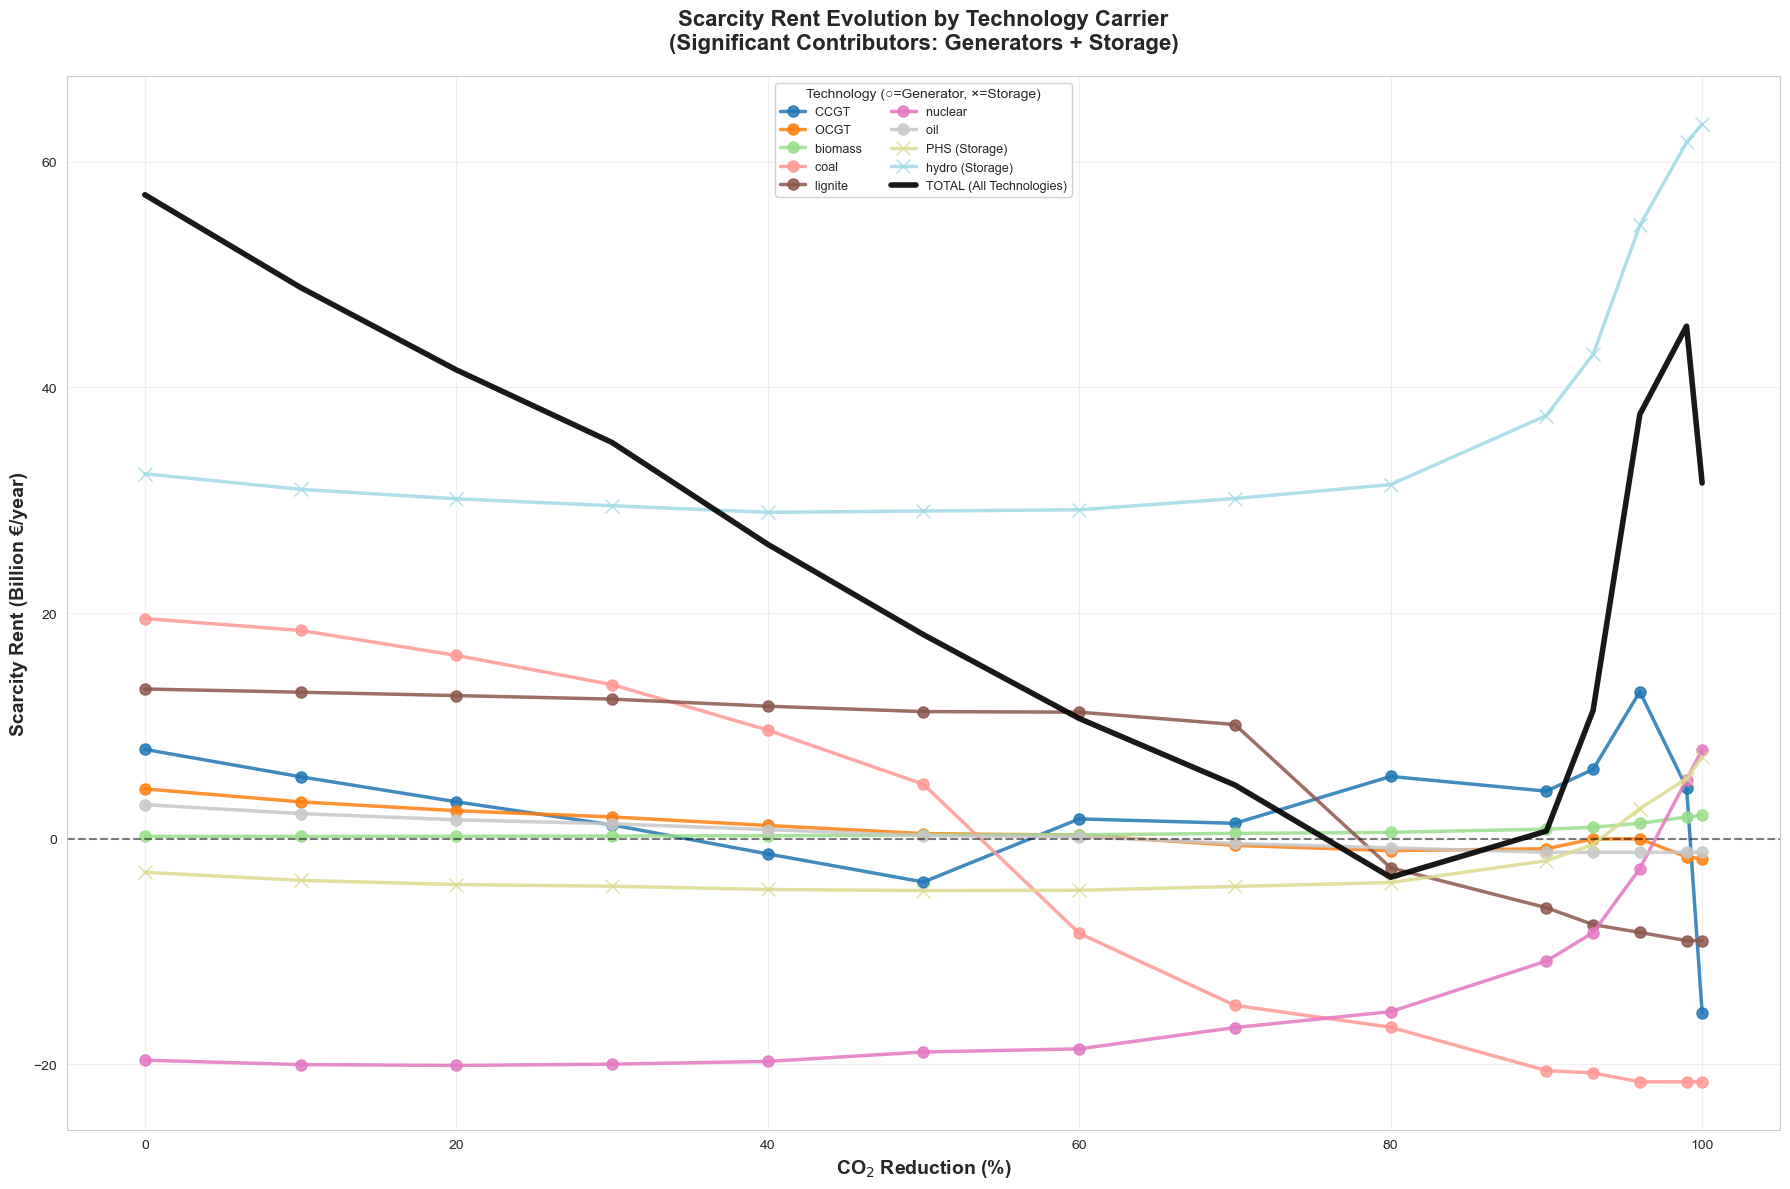
\includegraphics[width=\linewidth]{doc/scarcity_rent_evolution_contributions.png}
\caption{Scarcity rent contributions by technology}
\label{fig2}
\end{figure}

\medskip
\noindent
Here it can be seen that at low levels of decarbonization the majority of the contribution to the total scarcity rent comes from the fossil-fuel based generators. As the system decarbonizes the amount of fossil fuel generation is reduced in order to meet the decarbonization constraint and as such the contribution to the scarcity rent decreases. However at around 80\% decarbonization where the vast majority of the fossil based generation has been phased out, the main contributors become the dispatchable renewable generators, such as nuclear, and storage units needed for balancing.
This is illustrated in the modified version of Figure \ref{fig1} below:

\begin{figure}[H]
\centering
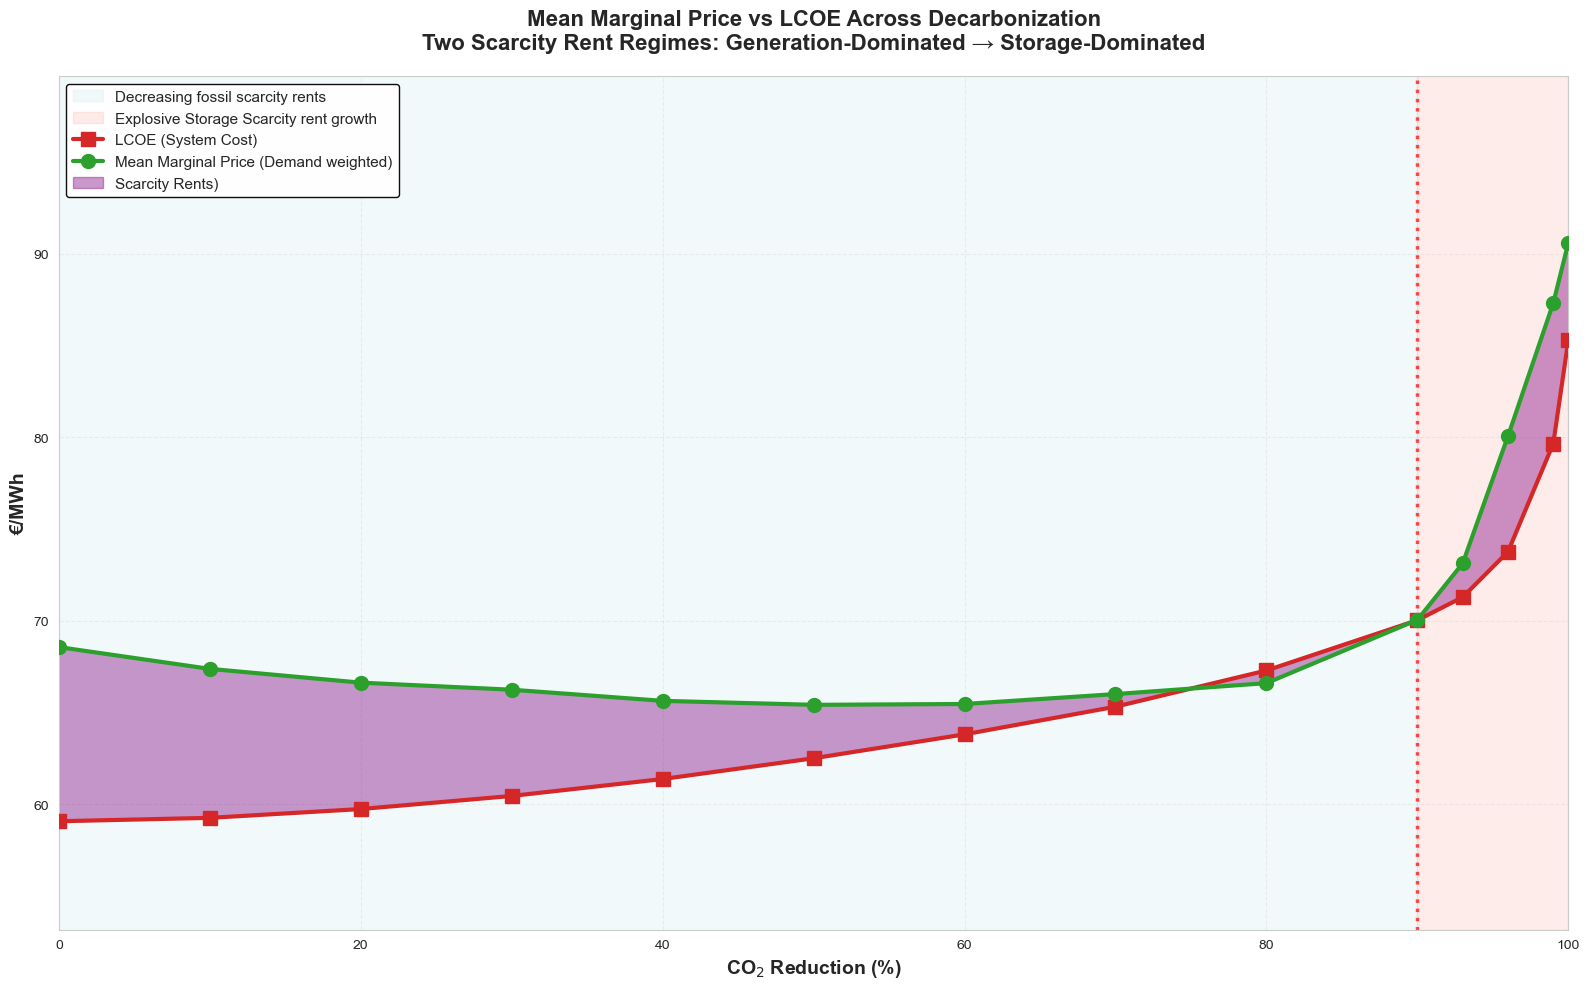
\includegraphics[width=\linewidth]{doc/Margnal_vs_LCOE_transition.png}
\caption{Transition between main scarcity rent contributors}
\label{fig3}
\end{figure}


\noindent
As a side note, a negative scarcity rent indicates that the technology in question is running at a loss, meaning that the revenue from selling electricity is not sufficient to cover the capital and marginal costs of the technology. One might think that such a technology would not be included in the optimized system, however as the optimization is performed on a brownfield system with existing capacity, it may be optimal to keep such a technology running at a loss if the overall system cost is reduced by doing so.

\medskip
\noindent
As for the initial decrease in mean marginal demand weighted price. This can be attributed to something called the "merit-order effect": When the decarbonization constraint of fossil fuel energy generation tightens, fossil-fuel based energy production is replaced by renewable generation. As some forms of renewable generation have very low marginal costs the mean marginal demand weighted price decreases as these low marginal cost generators set the market price in more snapshots. However the total system cost increases as the newly installed generation- and storage-capacity has capital costs that contribute to the overall increase in system cost as seen in Figure \ref{fig18} below:

\medskip
\noindent
\begin{figure}[H]
\centering
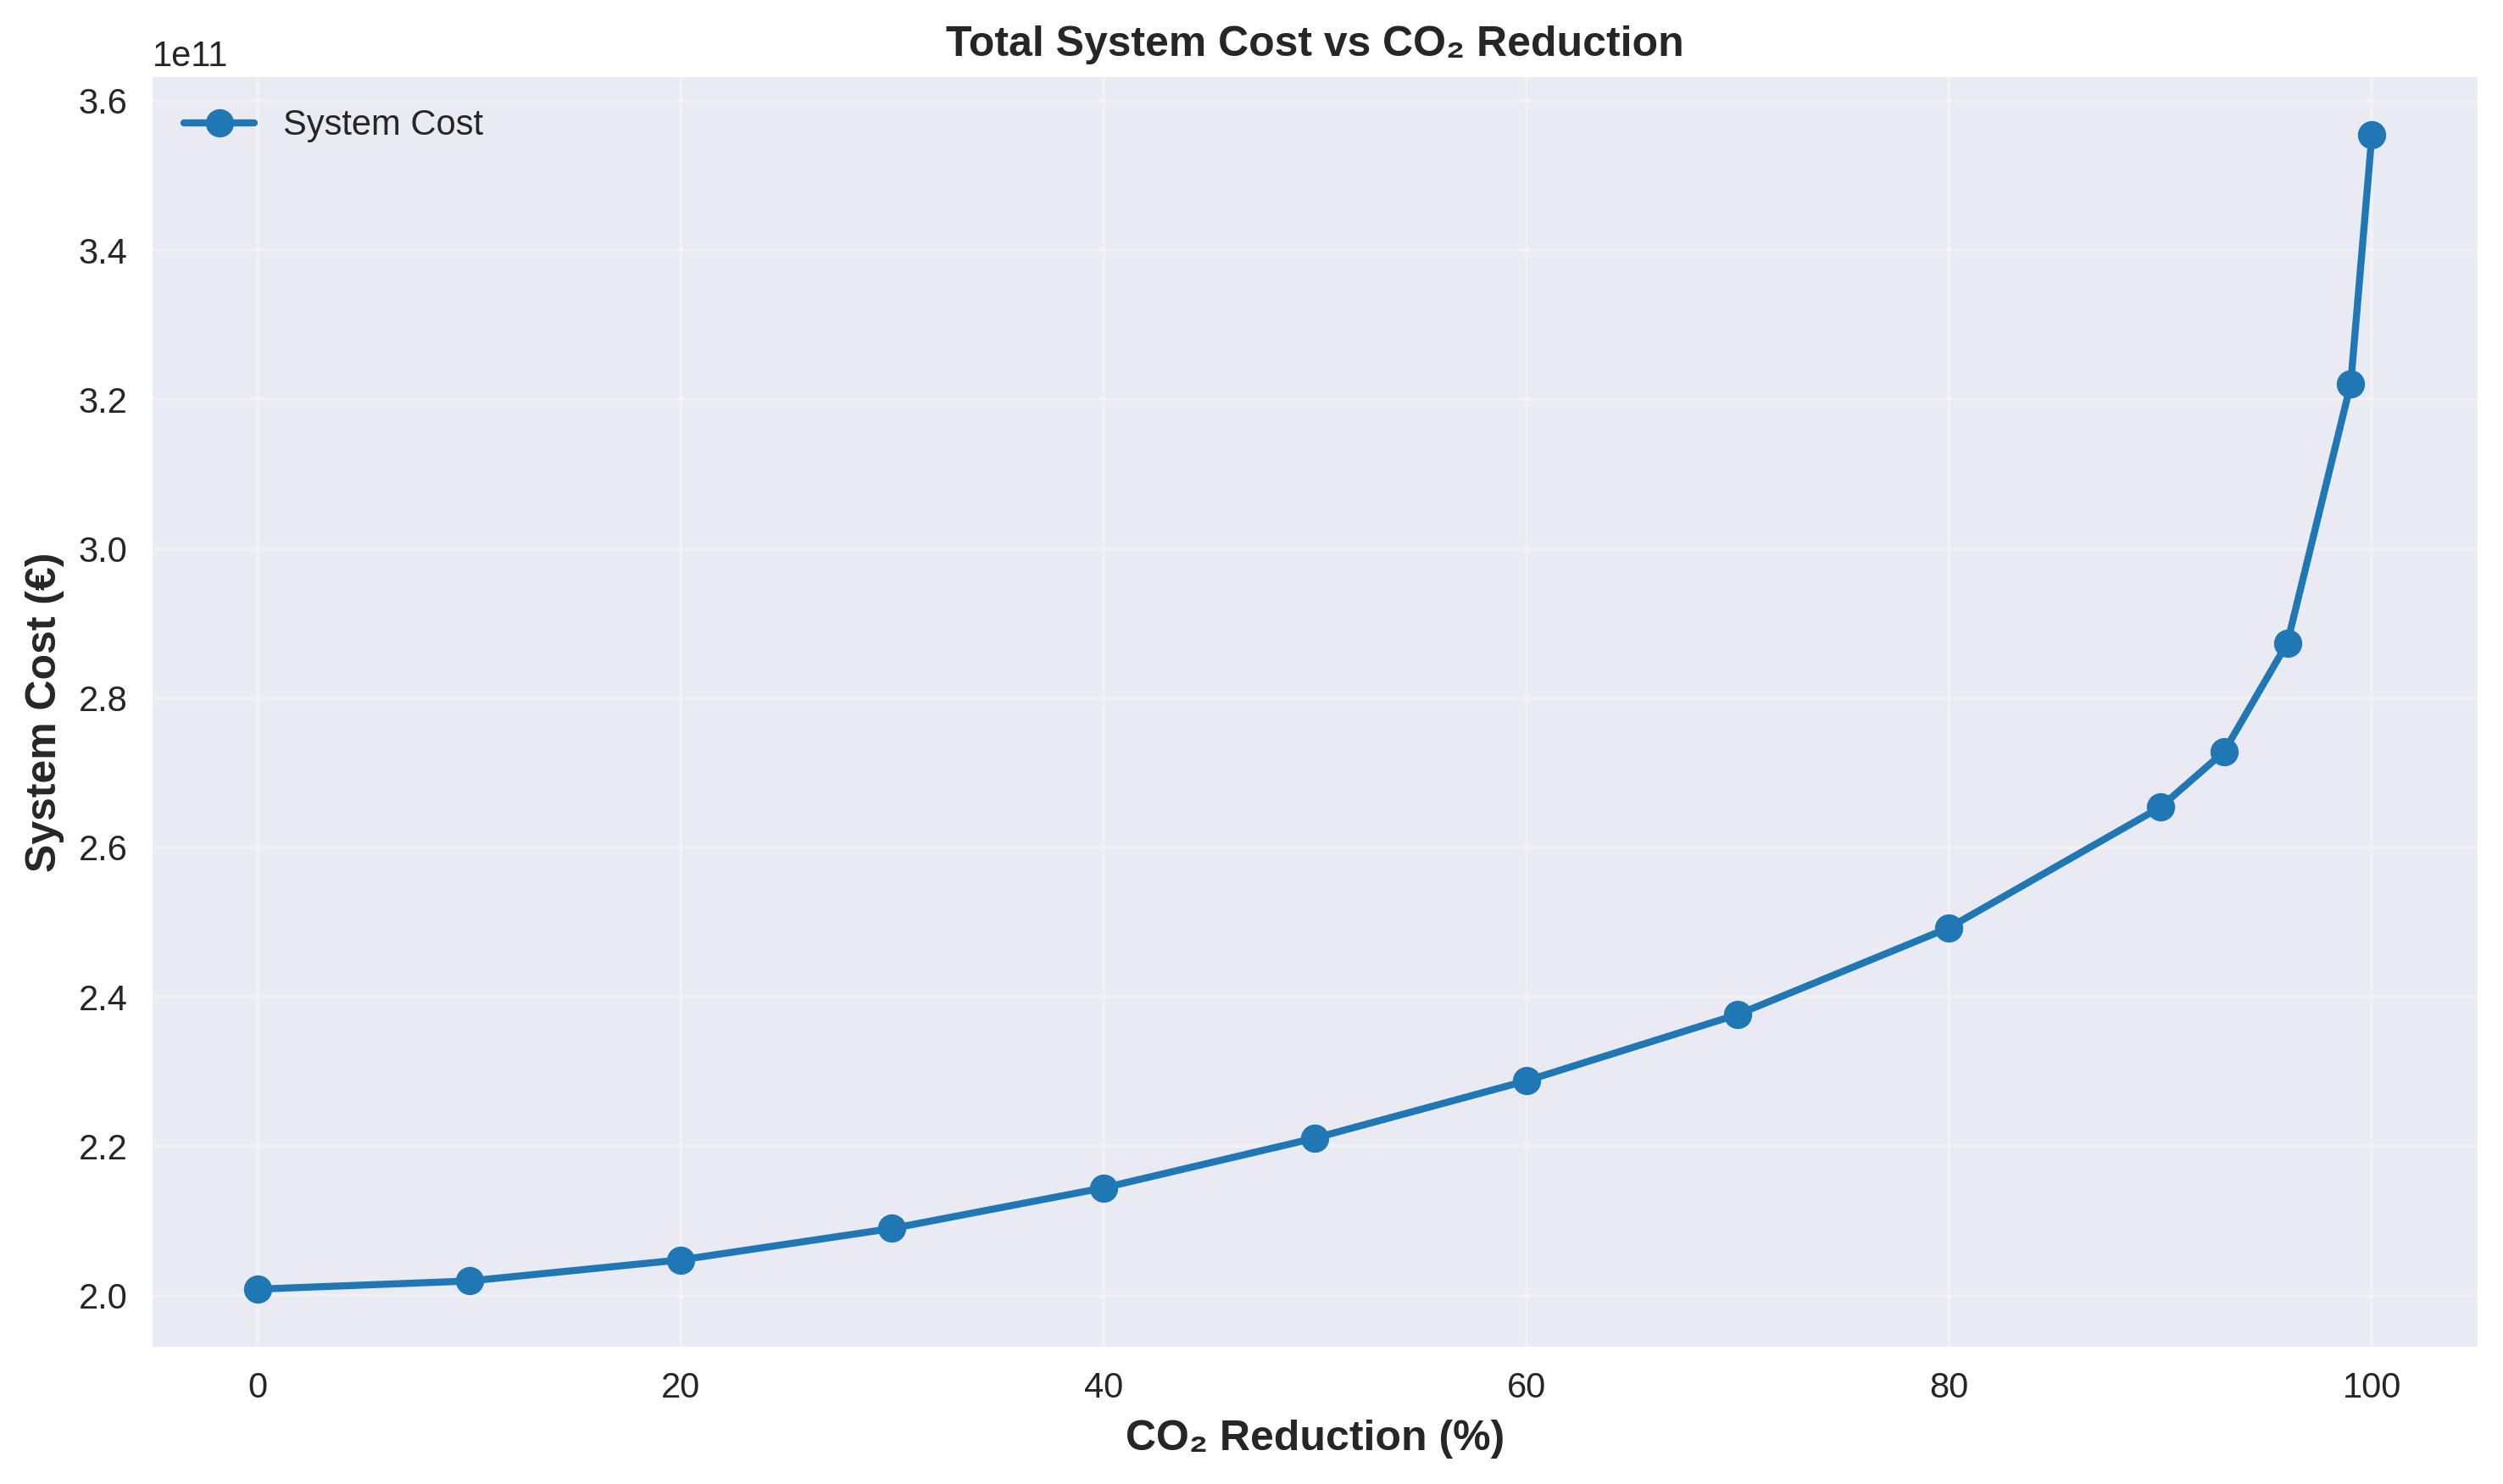
\includegraphics[width=\linewidth]{doc/SystemCost_K_infs.png}
\caption{Total system cost in least-cost systems}
\label{fig18}
\end{figure}

\begin{figure}[H]
\centering
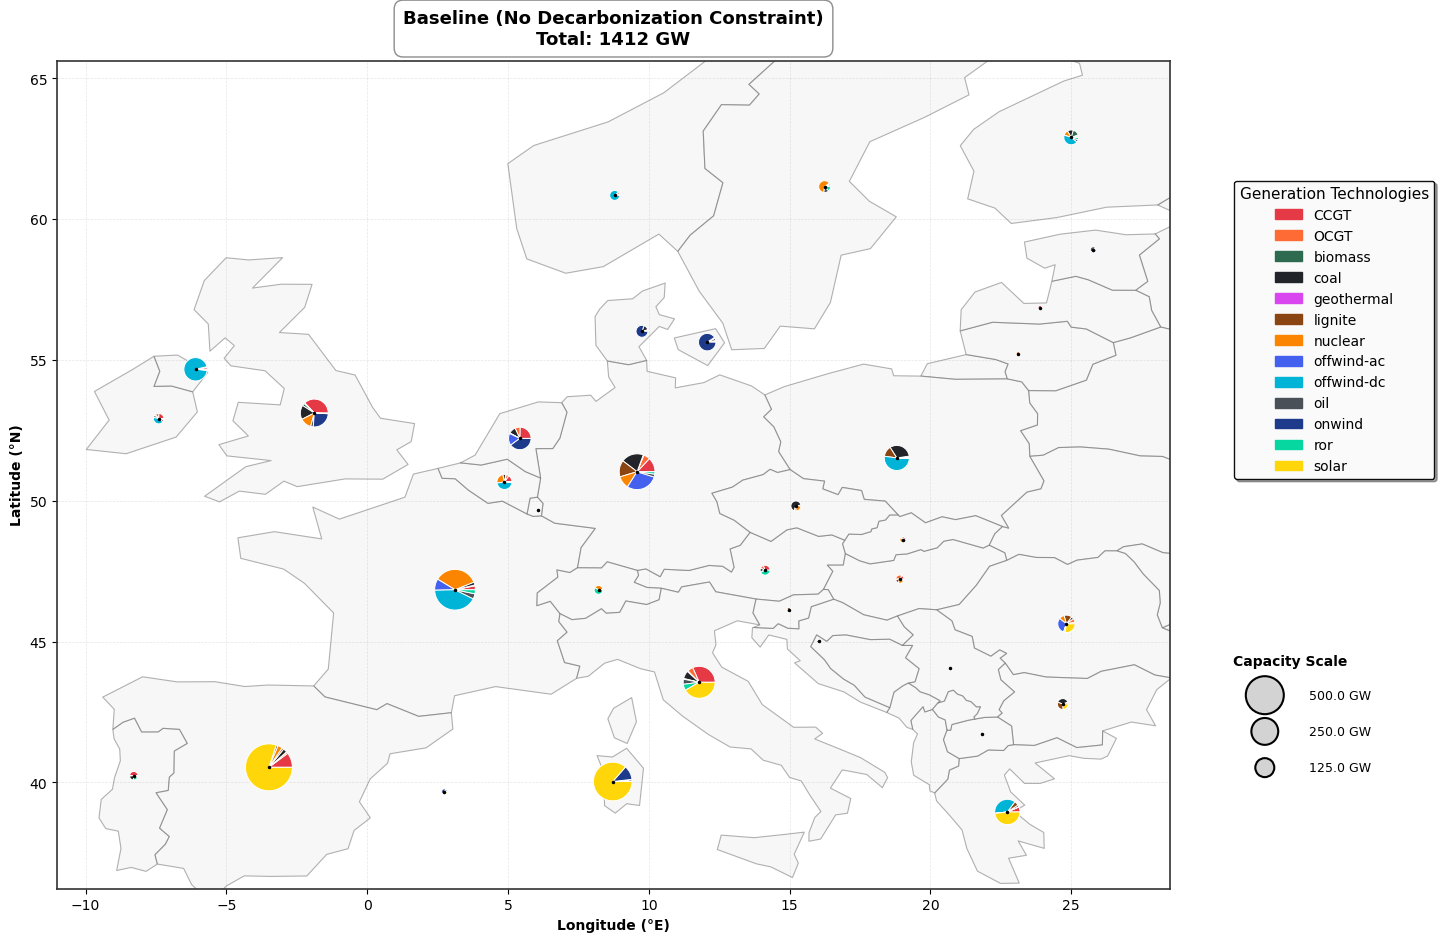
\includegraphics[width=\linewidth]{doc/CapacityMap_C0_K0.png}
\caption{Figure text}
\label{fig4}
\end{figure}


\begin{figure}[H]
\centering
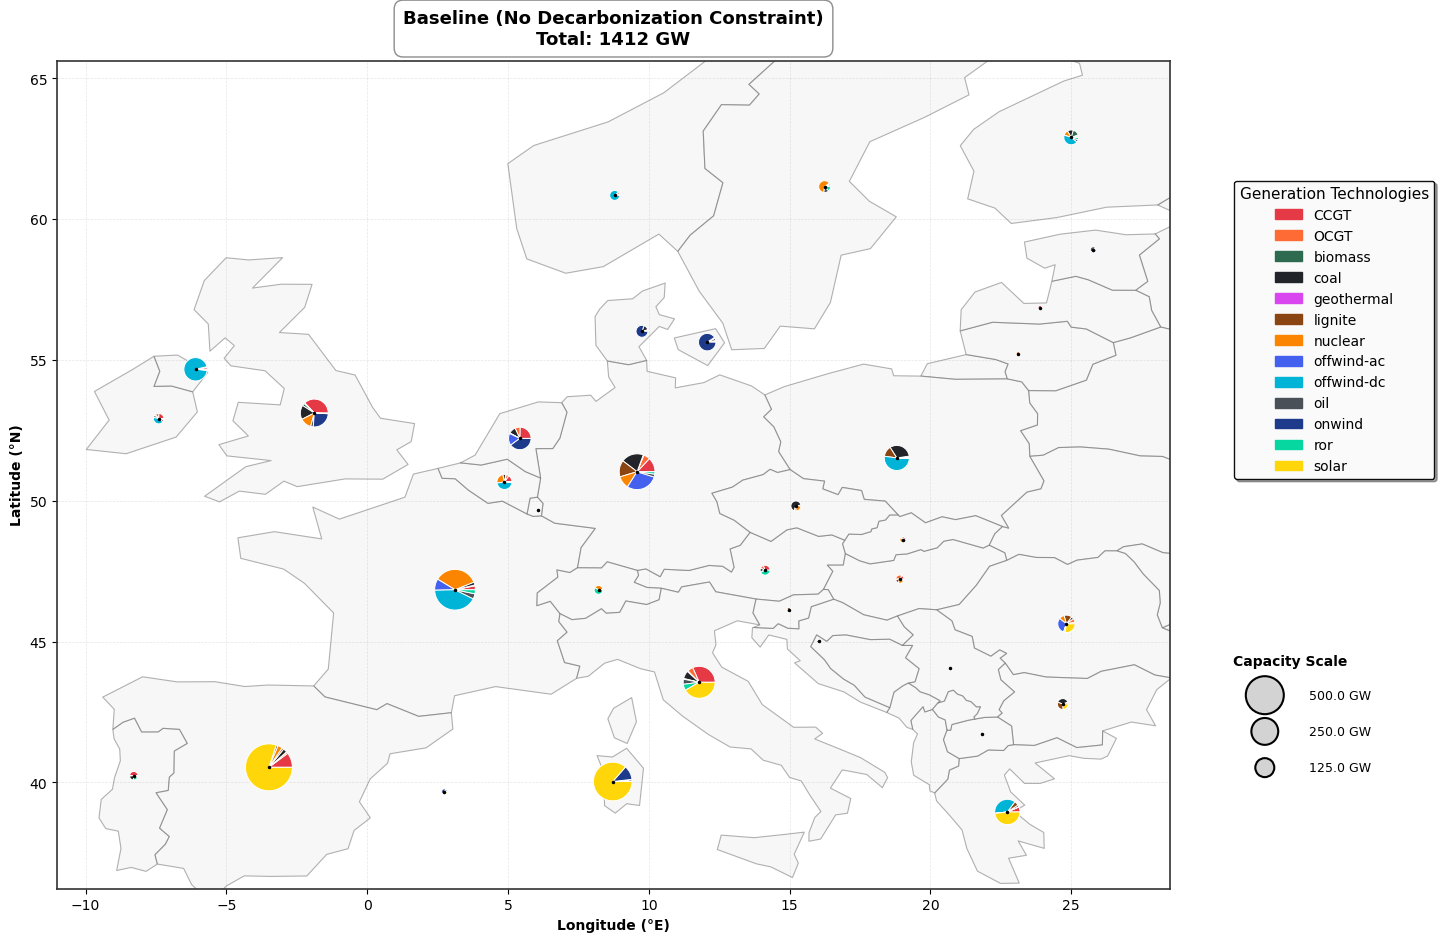
\includegraphics[width=\linewidth]{doc/CapacityMap_C0_K0.png}
\caption{Figure text}
\label{fig5}
\end{figure}

\medskip
\noindent
\begin{figure}[H]
\centering
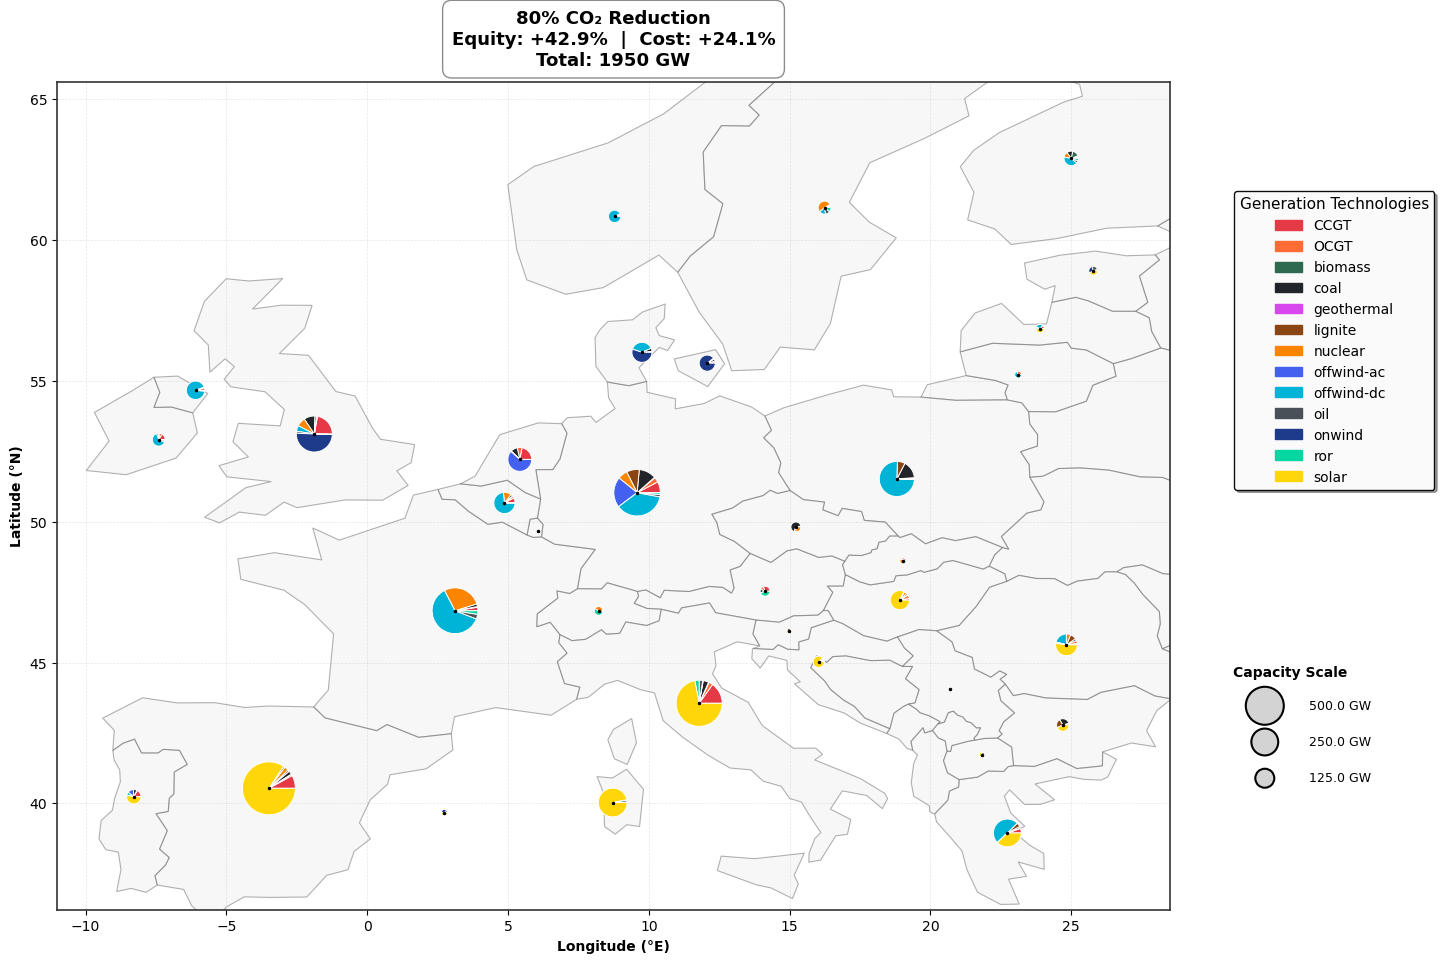
\includegraphics[width=\linewidth]{doc/CapacityMap_C80_K0.png}
\caption{Figure text}
\label{fig6}
\end{figure}

\medskip
\noindent
\begin{figure}[H]
\centering
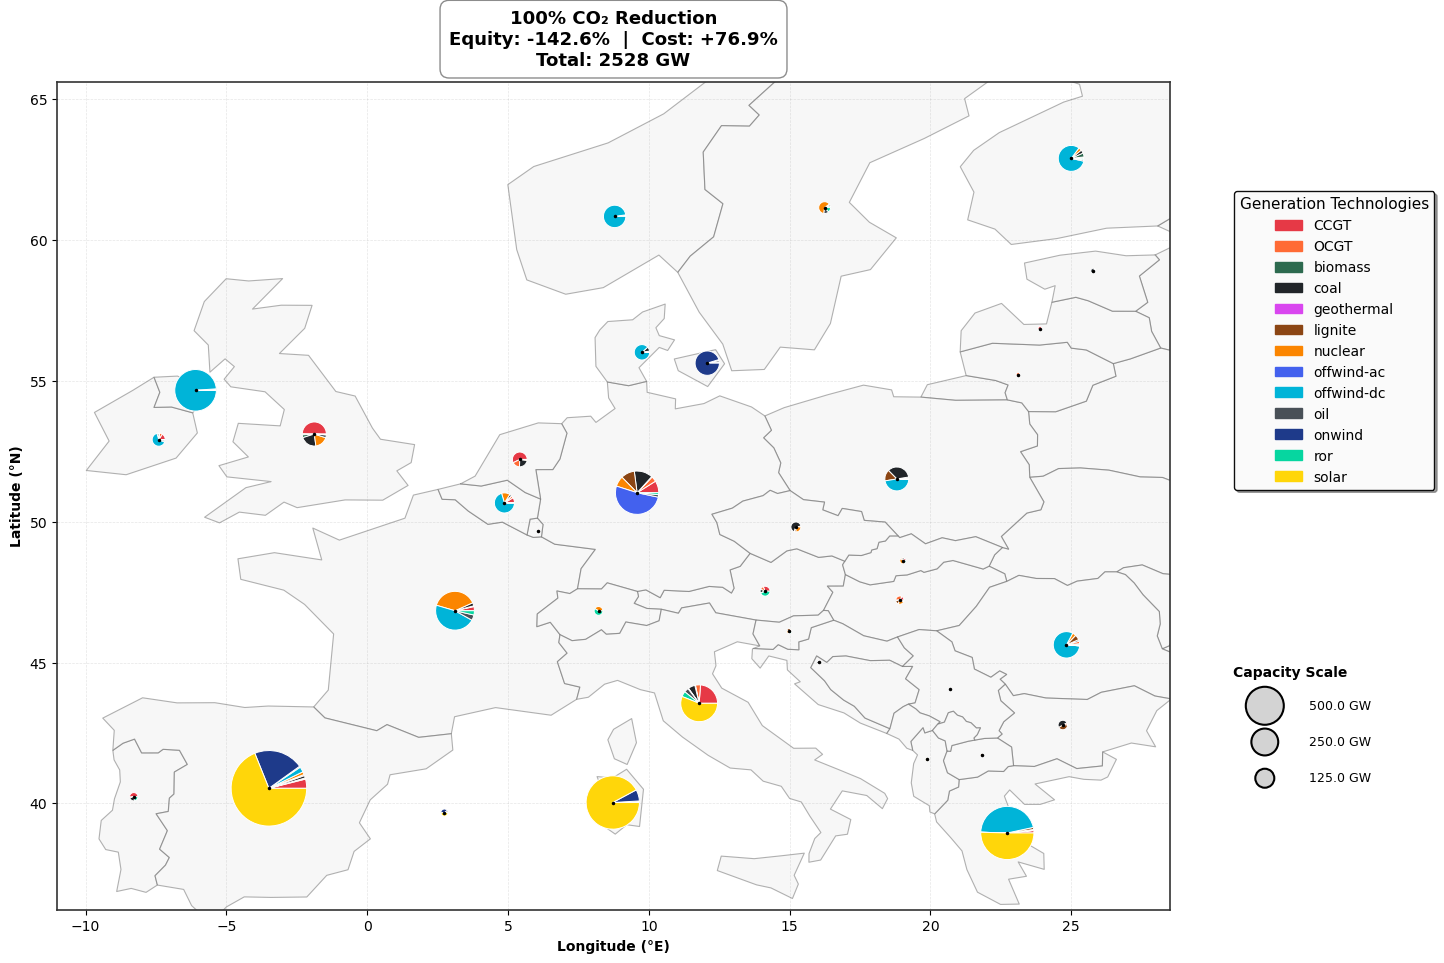
\includegraphics[width=\linewidth]{doc/CapacityMap_C100_K0.png}
\caption{Figure text}
\label{fig7}
\end{figure}

\medskip
\noindent
\begin{figure}[H]
\centering
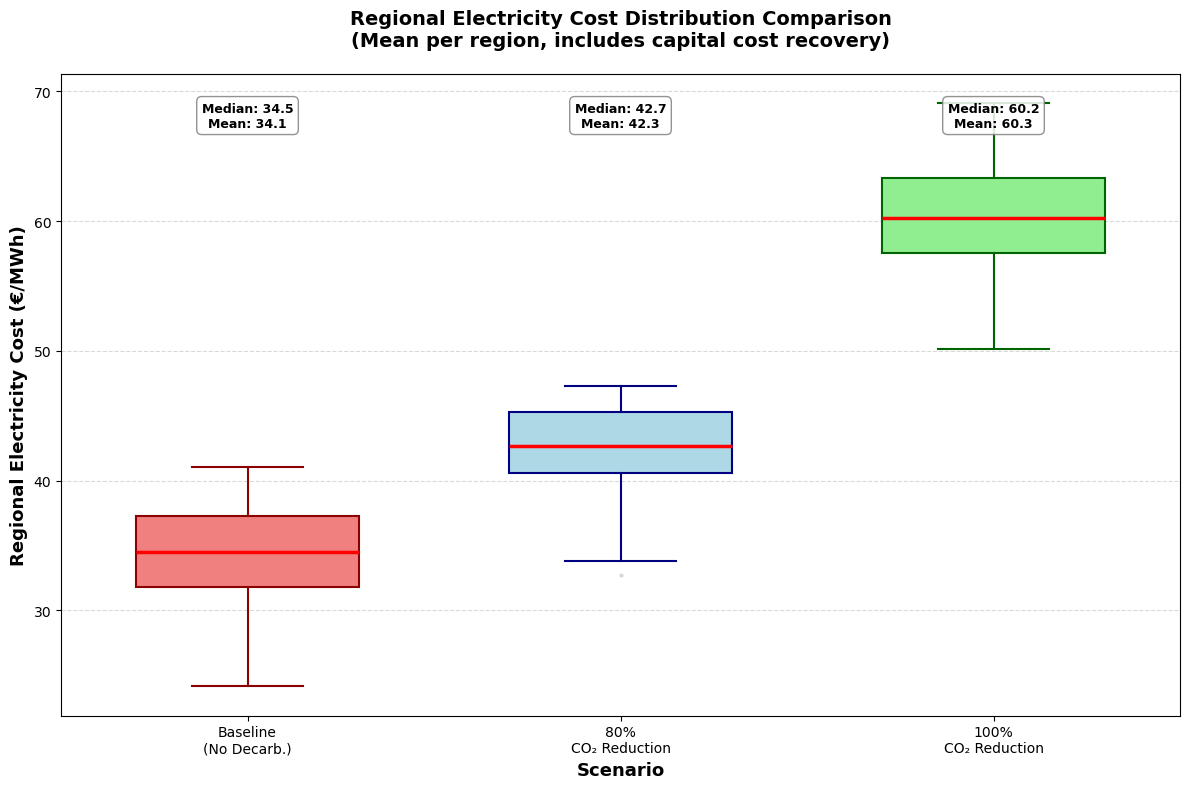
\includegraphics[width=\linewidth]{doc/RegionalElectricityPrice_C100_80_0_K_0.png}
\caption{Figure text}
\label{fig8}
\end{figure}

\medskip
\noindent
\begin{figure}[H]
\centering
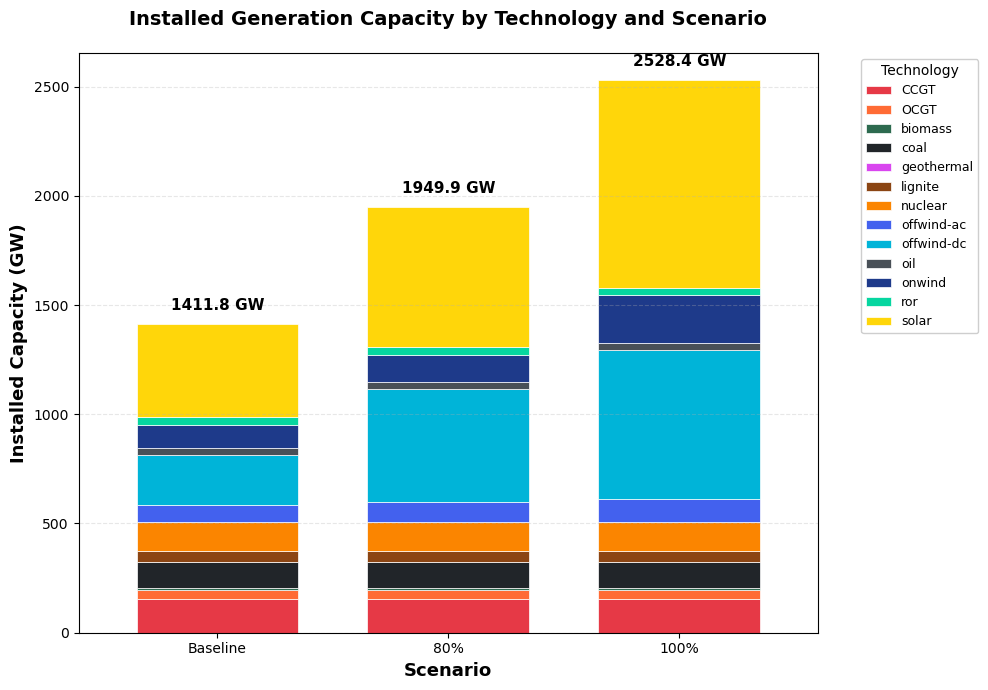
\includegraphics[width=\linewidth]{doc/GenerationCapacityStackedBar_C100_80_0_K0.png}
\caption{Figure text}
\label{fig9}
\end{figure}

\medskip
\noindent
\begin{figure}[H]
\centering
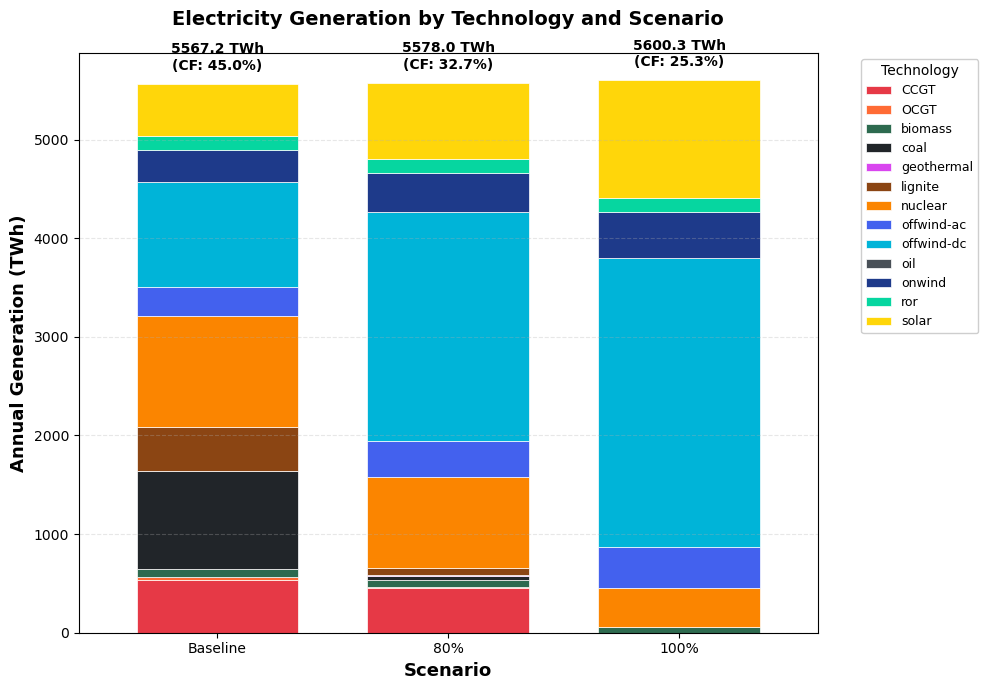
\includegraphics[width=\linewidth]{doc/GenerationStackedBar_C100_80_0_K0.png}
\caption{Figure text}
\label{fig10}
\end{figure}

\medskip
\noindent
\begin{figure}[H]
\centering
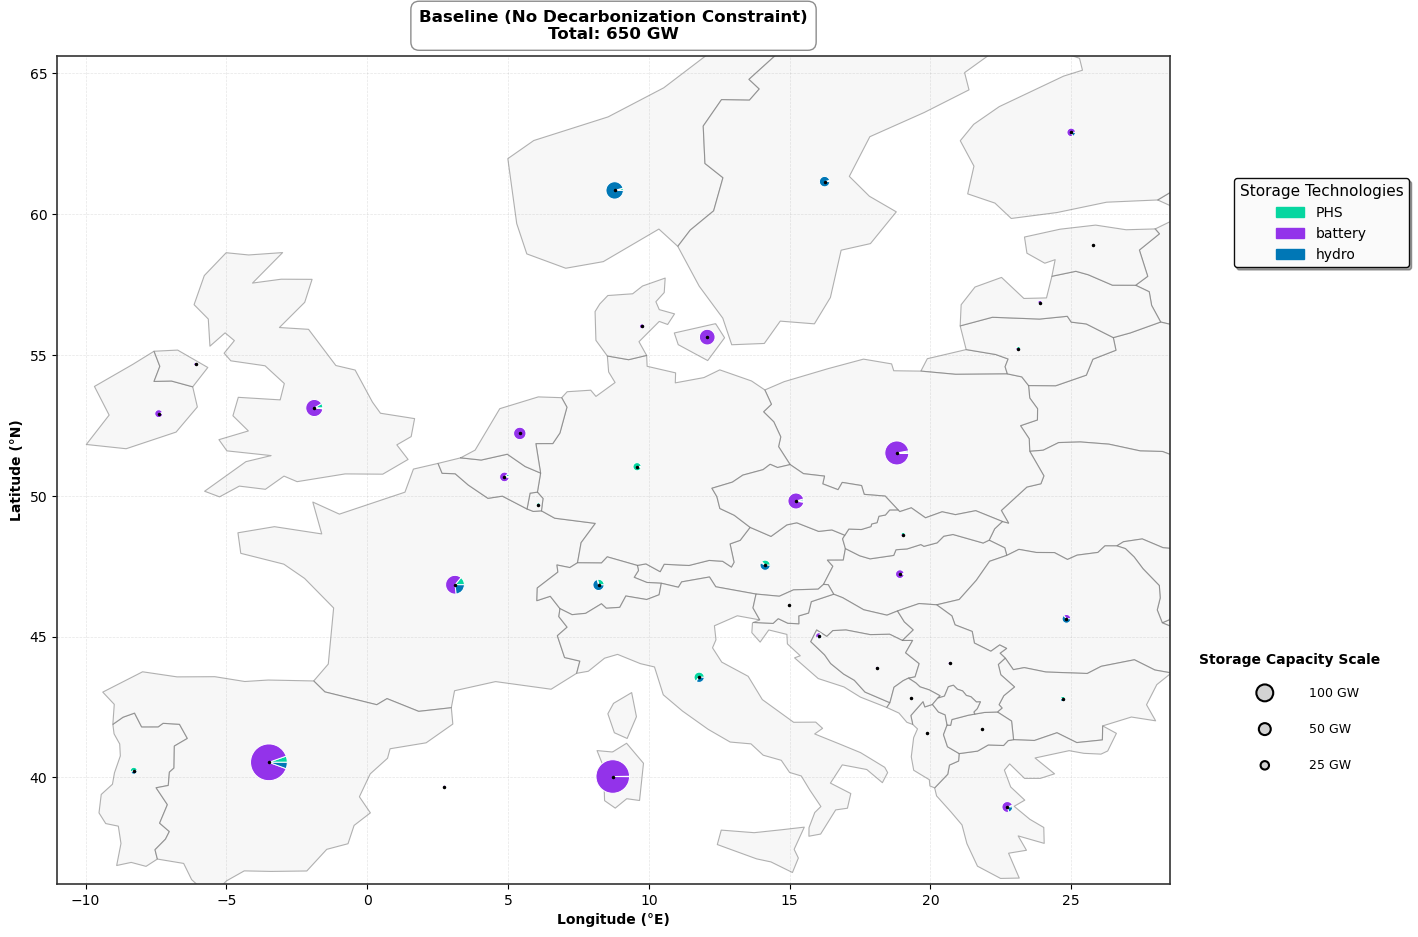
\includegraphics[width=\linewidth]{doc/StorageCapacityMap_C0_K0.png}
\caption{Figure text}
\label{fig11}
\end{figure}

\medskip
\noindent
\begin{figure}[H]
\centering
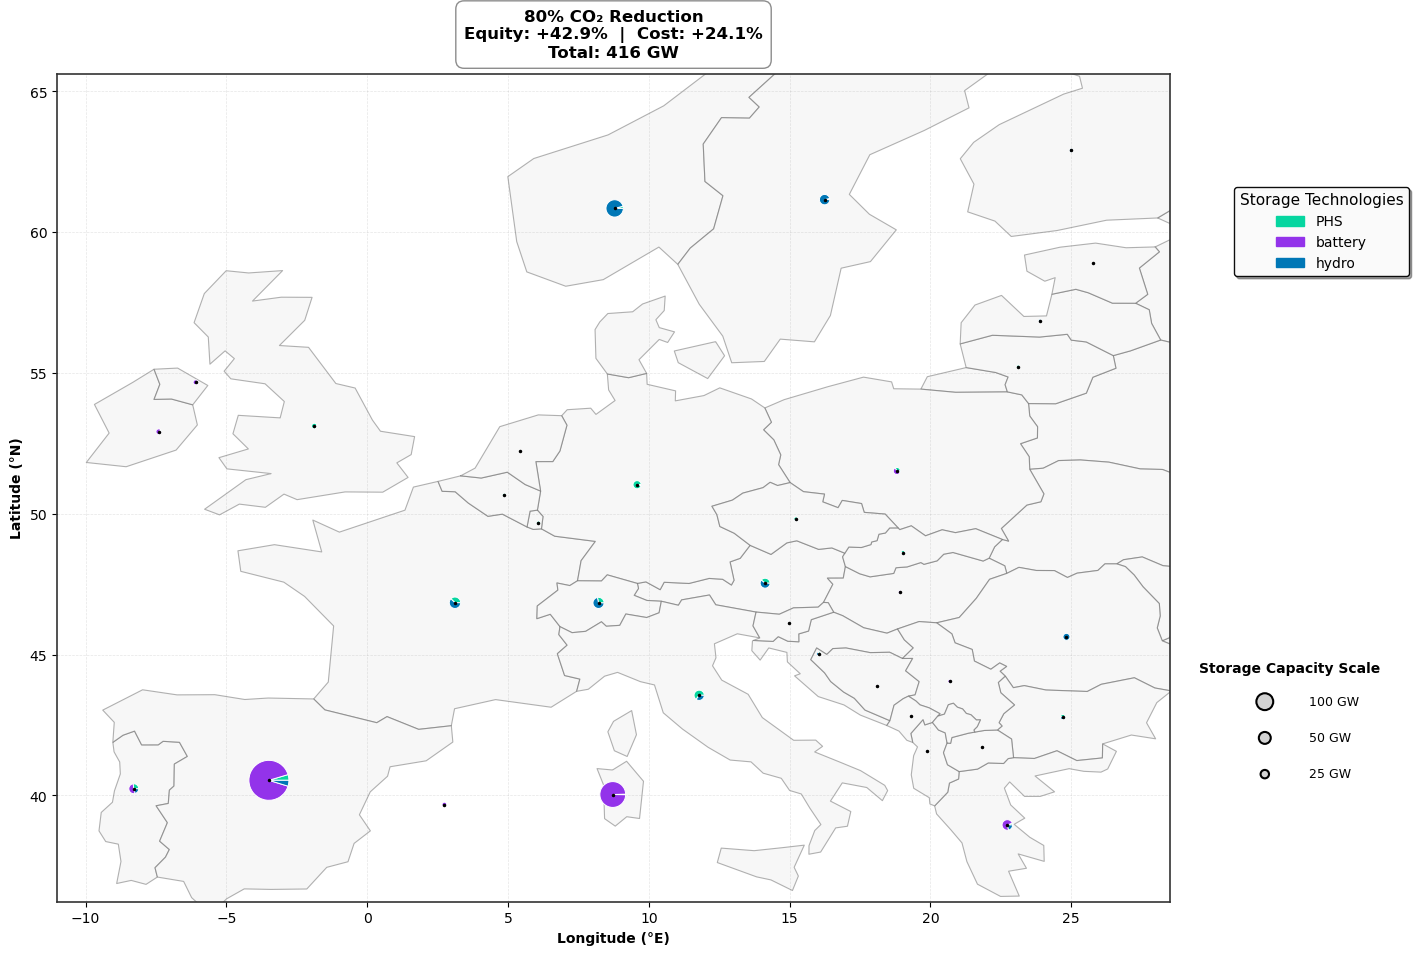
\includegraphics[width=\linewidth]{doc/StorageCapacityMap_C80_K0.png}
\caption{Figure text}
\label{fig12}
\end{figure}

\medskip
\noindent
\begin{figure}[H]
\centering
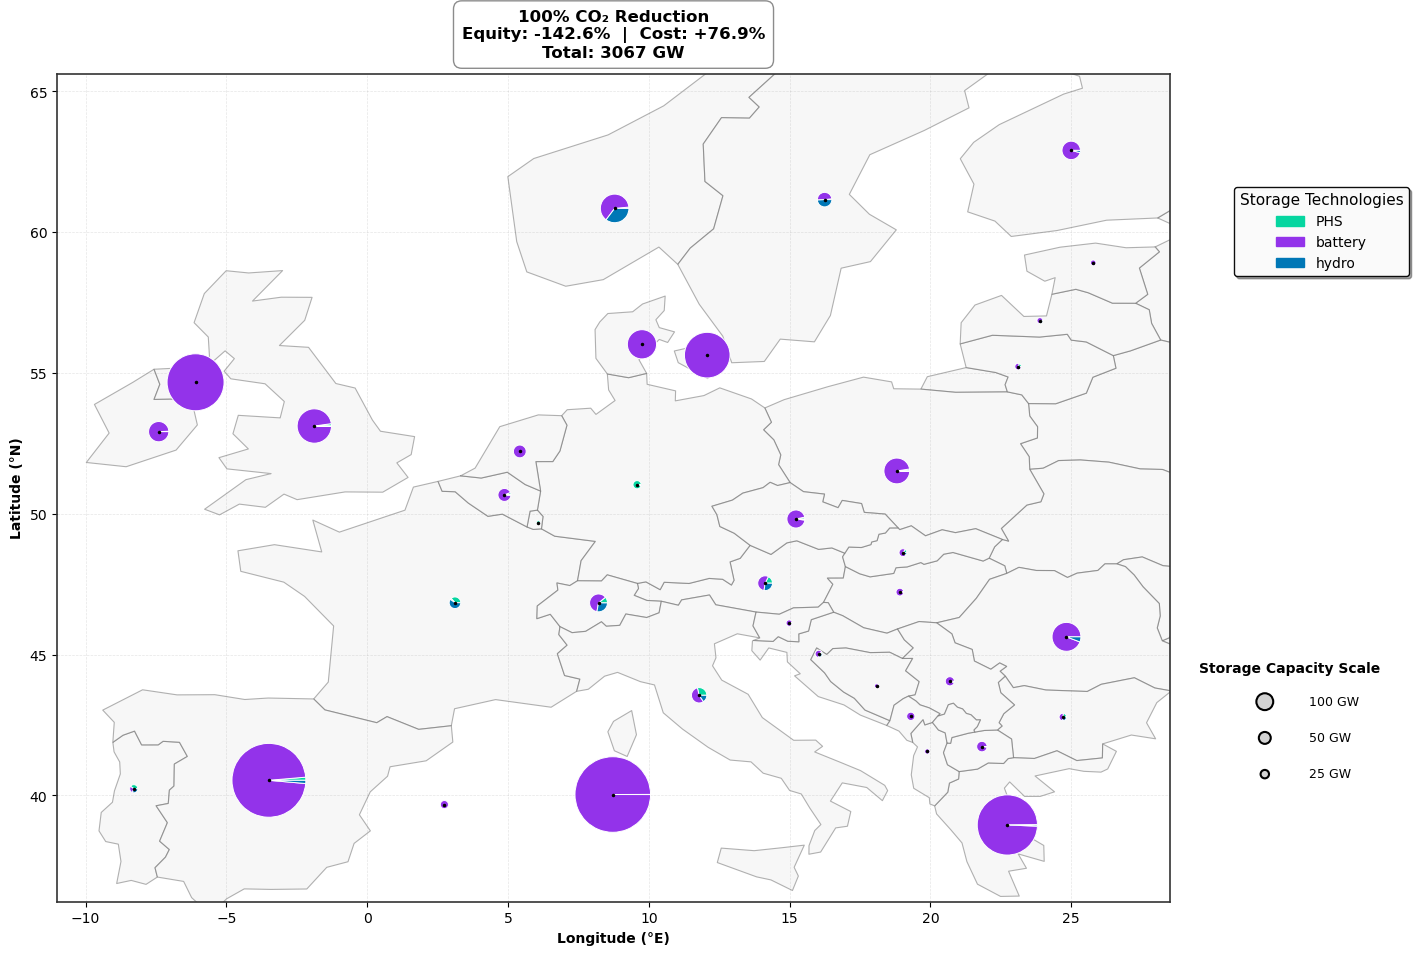
\includegraphics[width=\linewidth]{doc/StorageCapacityMap_C100_K0.png}
\caption{Figure text}
\label{fig13}
\end{figure}

\medskip
\noindent
\begin{figure}[H]
\centering
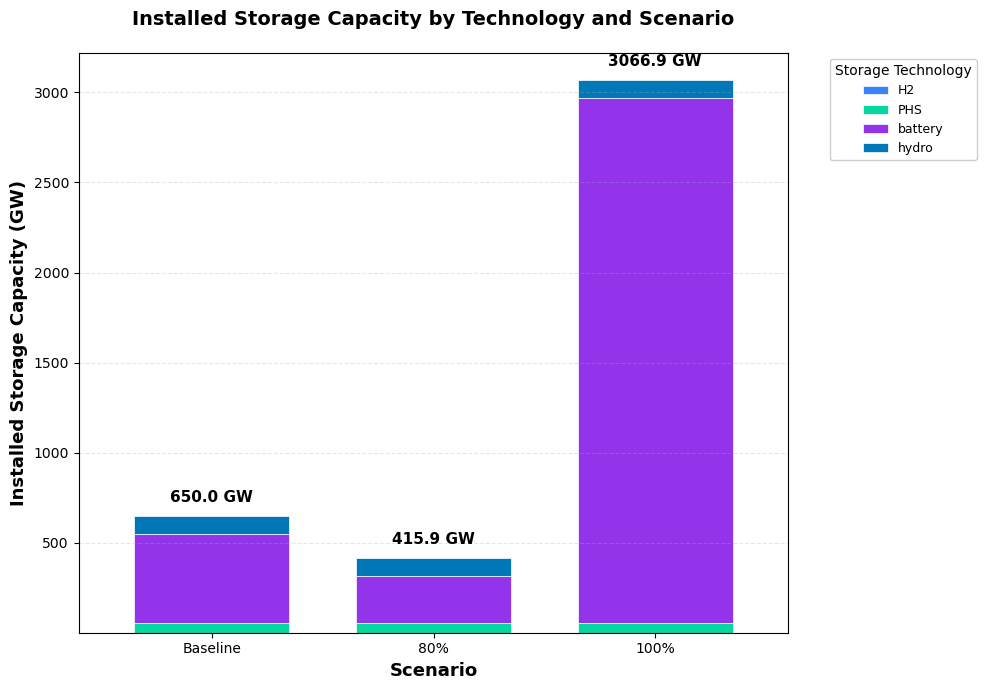
\includegraphics[width=\linewidth]{doc/StorageCapacityStackedBar_C100_80_0_K0.png}
\caption{Figure text}
\label{fig14}
\end{figure}

\subsubsection{Sanity checks and validations}
Comparing systems to real systems
\subsubsection{Decarbonization trends}
Analyzing trends in key figures and plots for the decarbonizing systems

\medskip
\noindent
\begin{figure}[H]
\centering
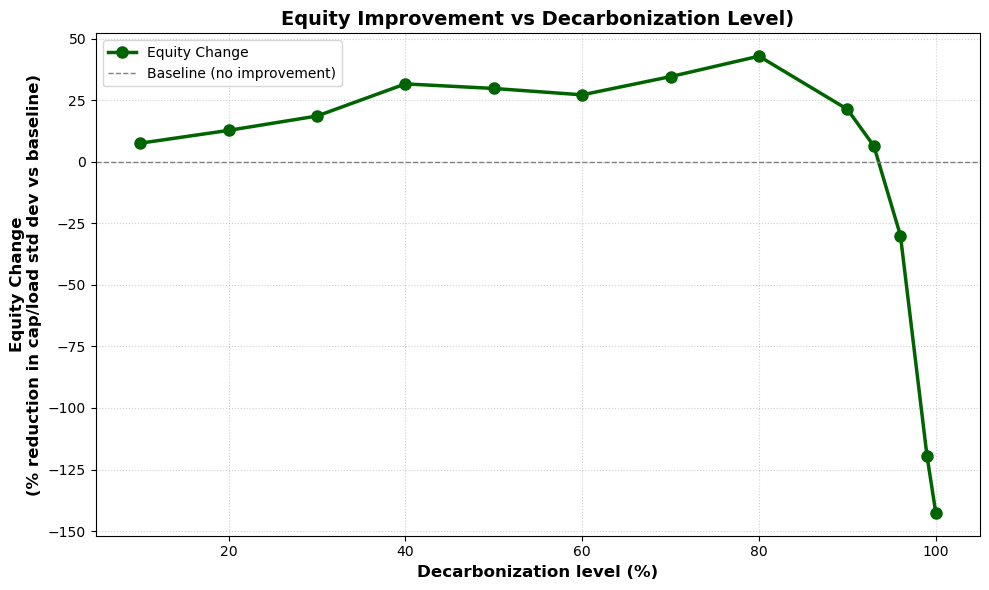
\includegraphics[width=\linewidth]{doc/EquityChange_K_infs.png}
\caption{Figure text}
\label{fig15}
\end{figure}

\medskip
\noindent
\begin{figure}[H]
\centering
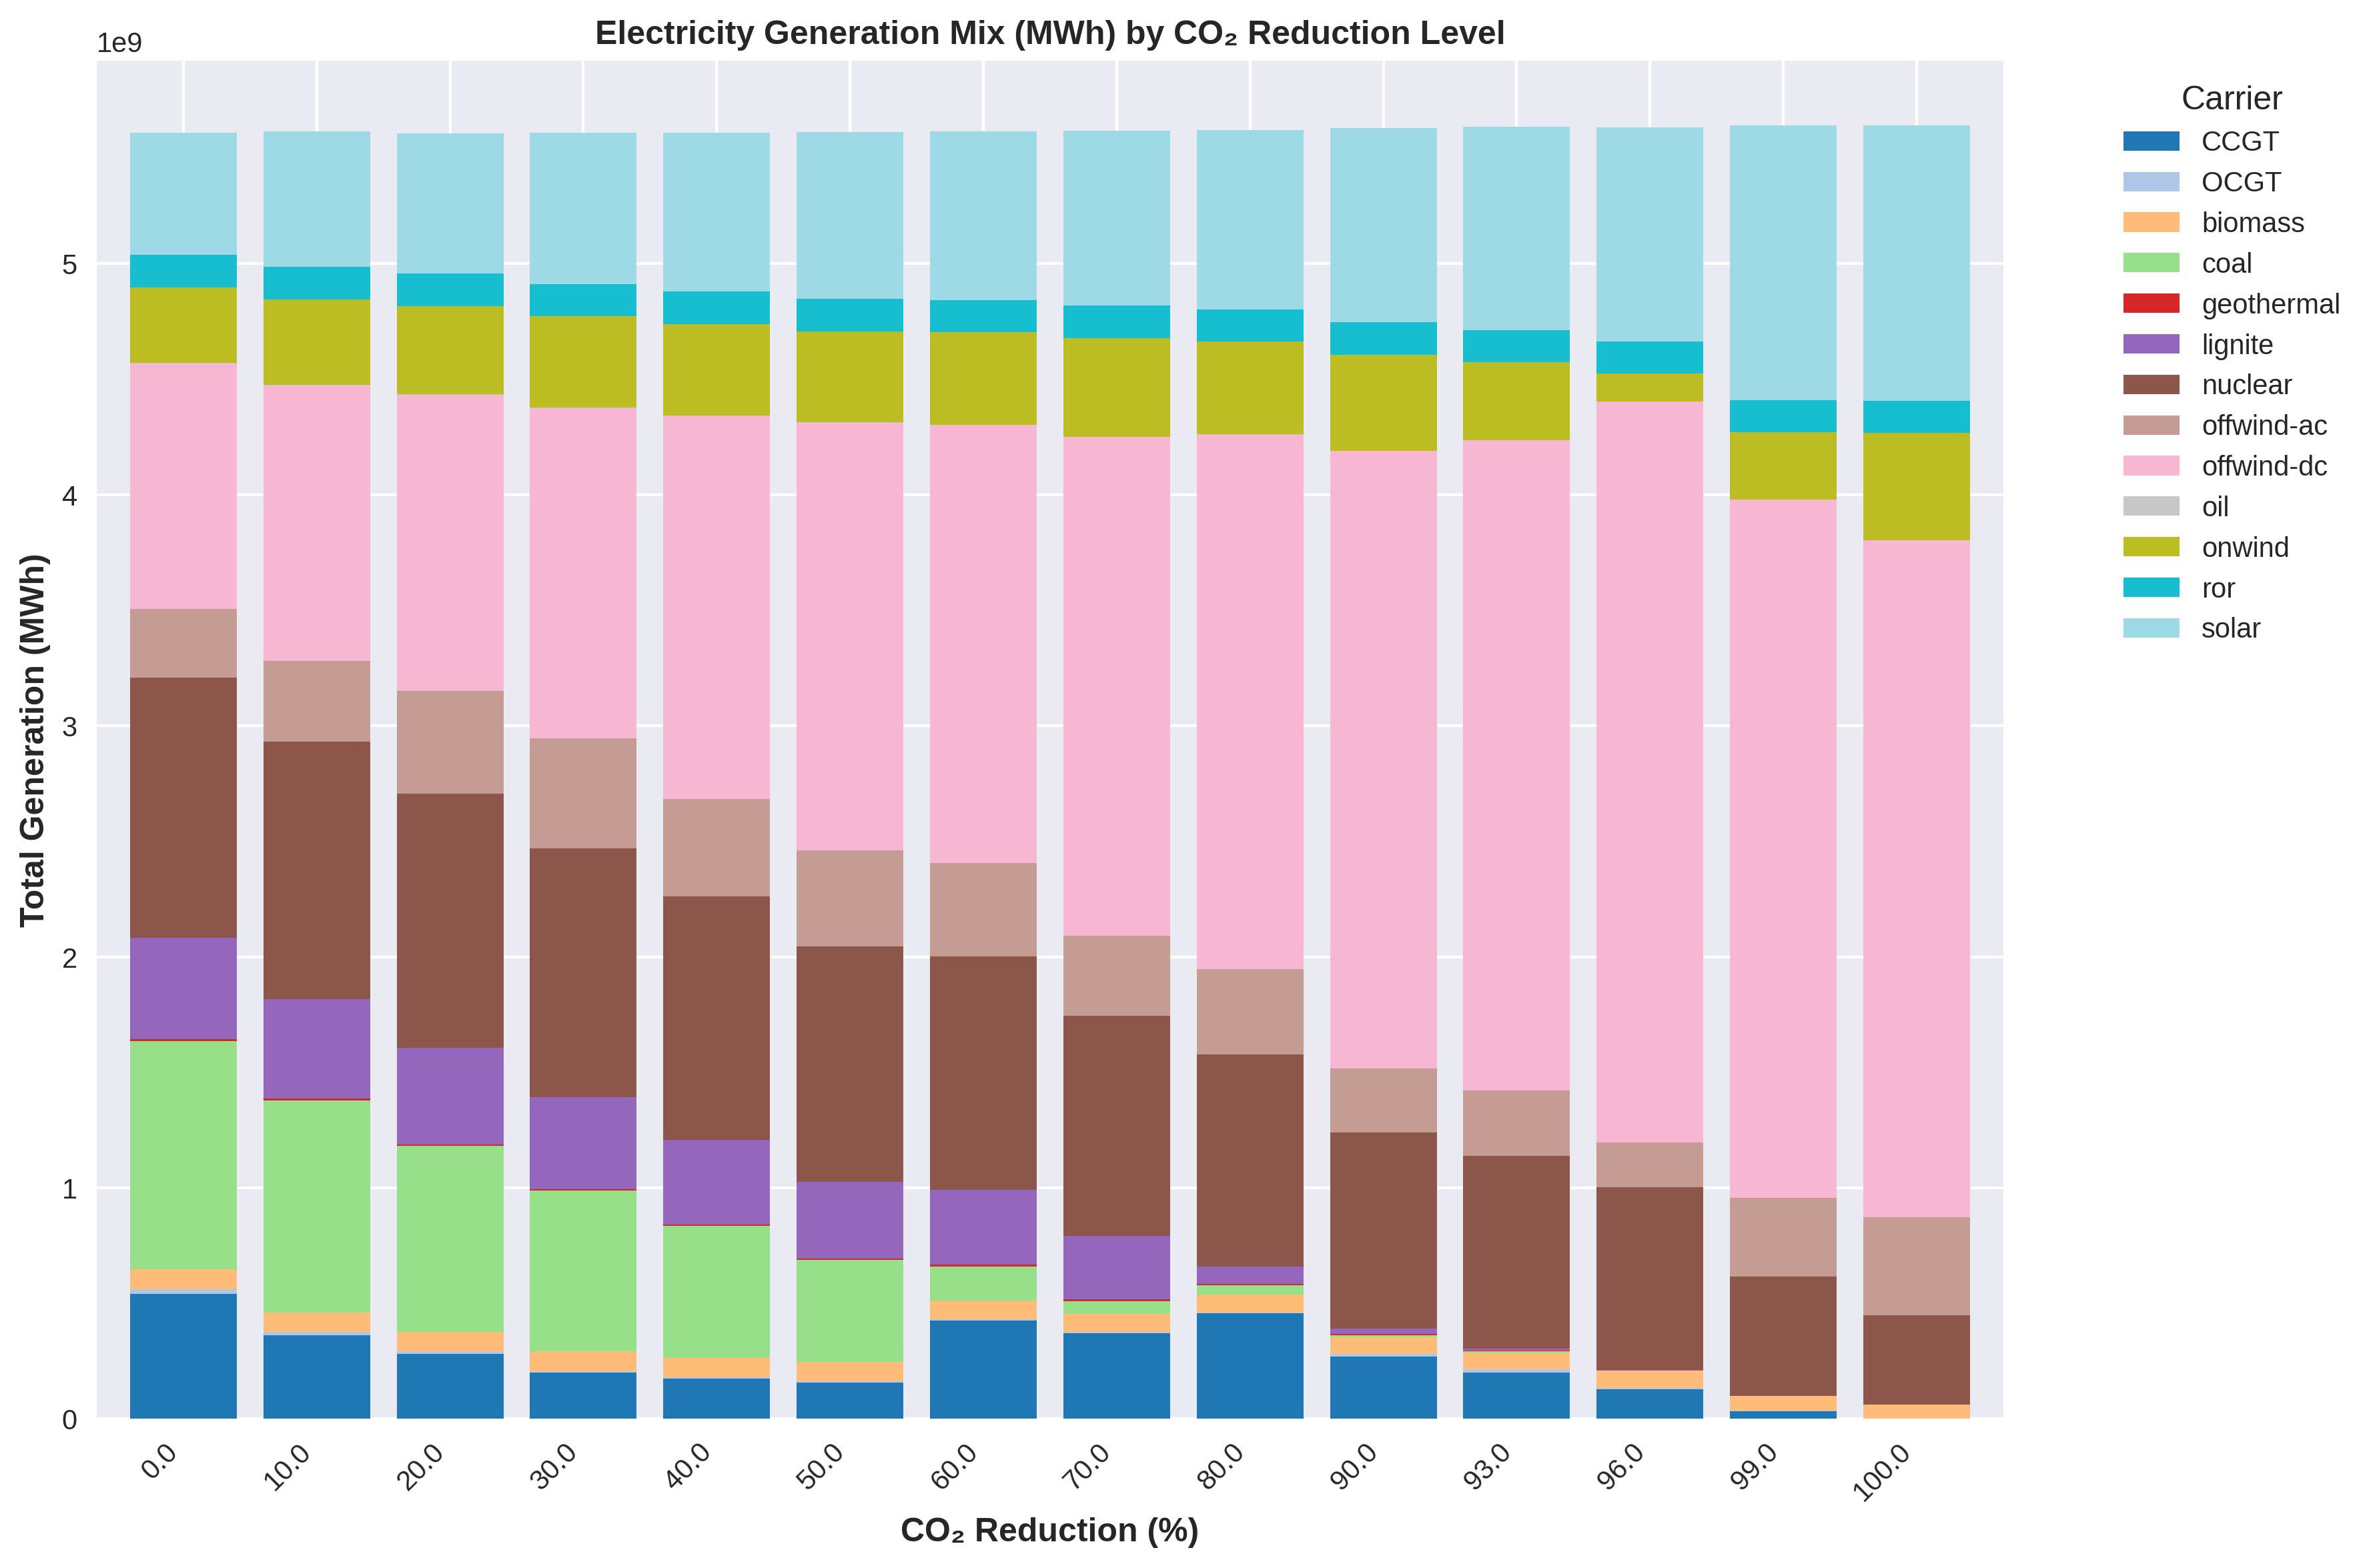
\includegraphics[width=\linewidth]{doc/GenerationStackedBar_K_infs.png}
\caption{Figure text}
\label{fig16}
\end{figure}

\medskip
\noindent
\begin{figure}[H]
\centering
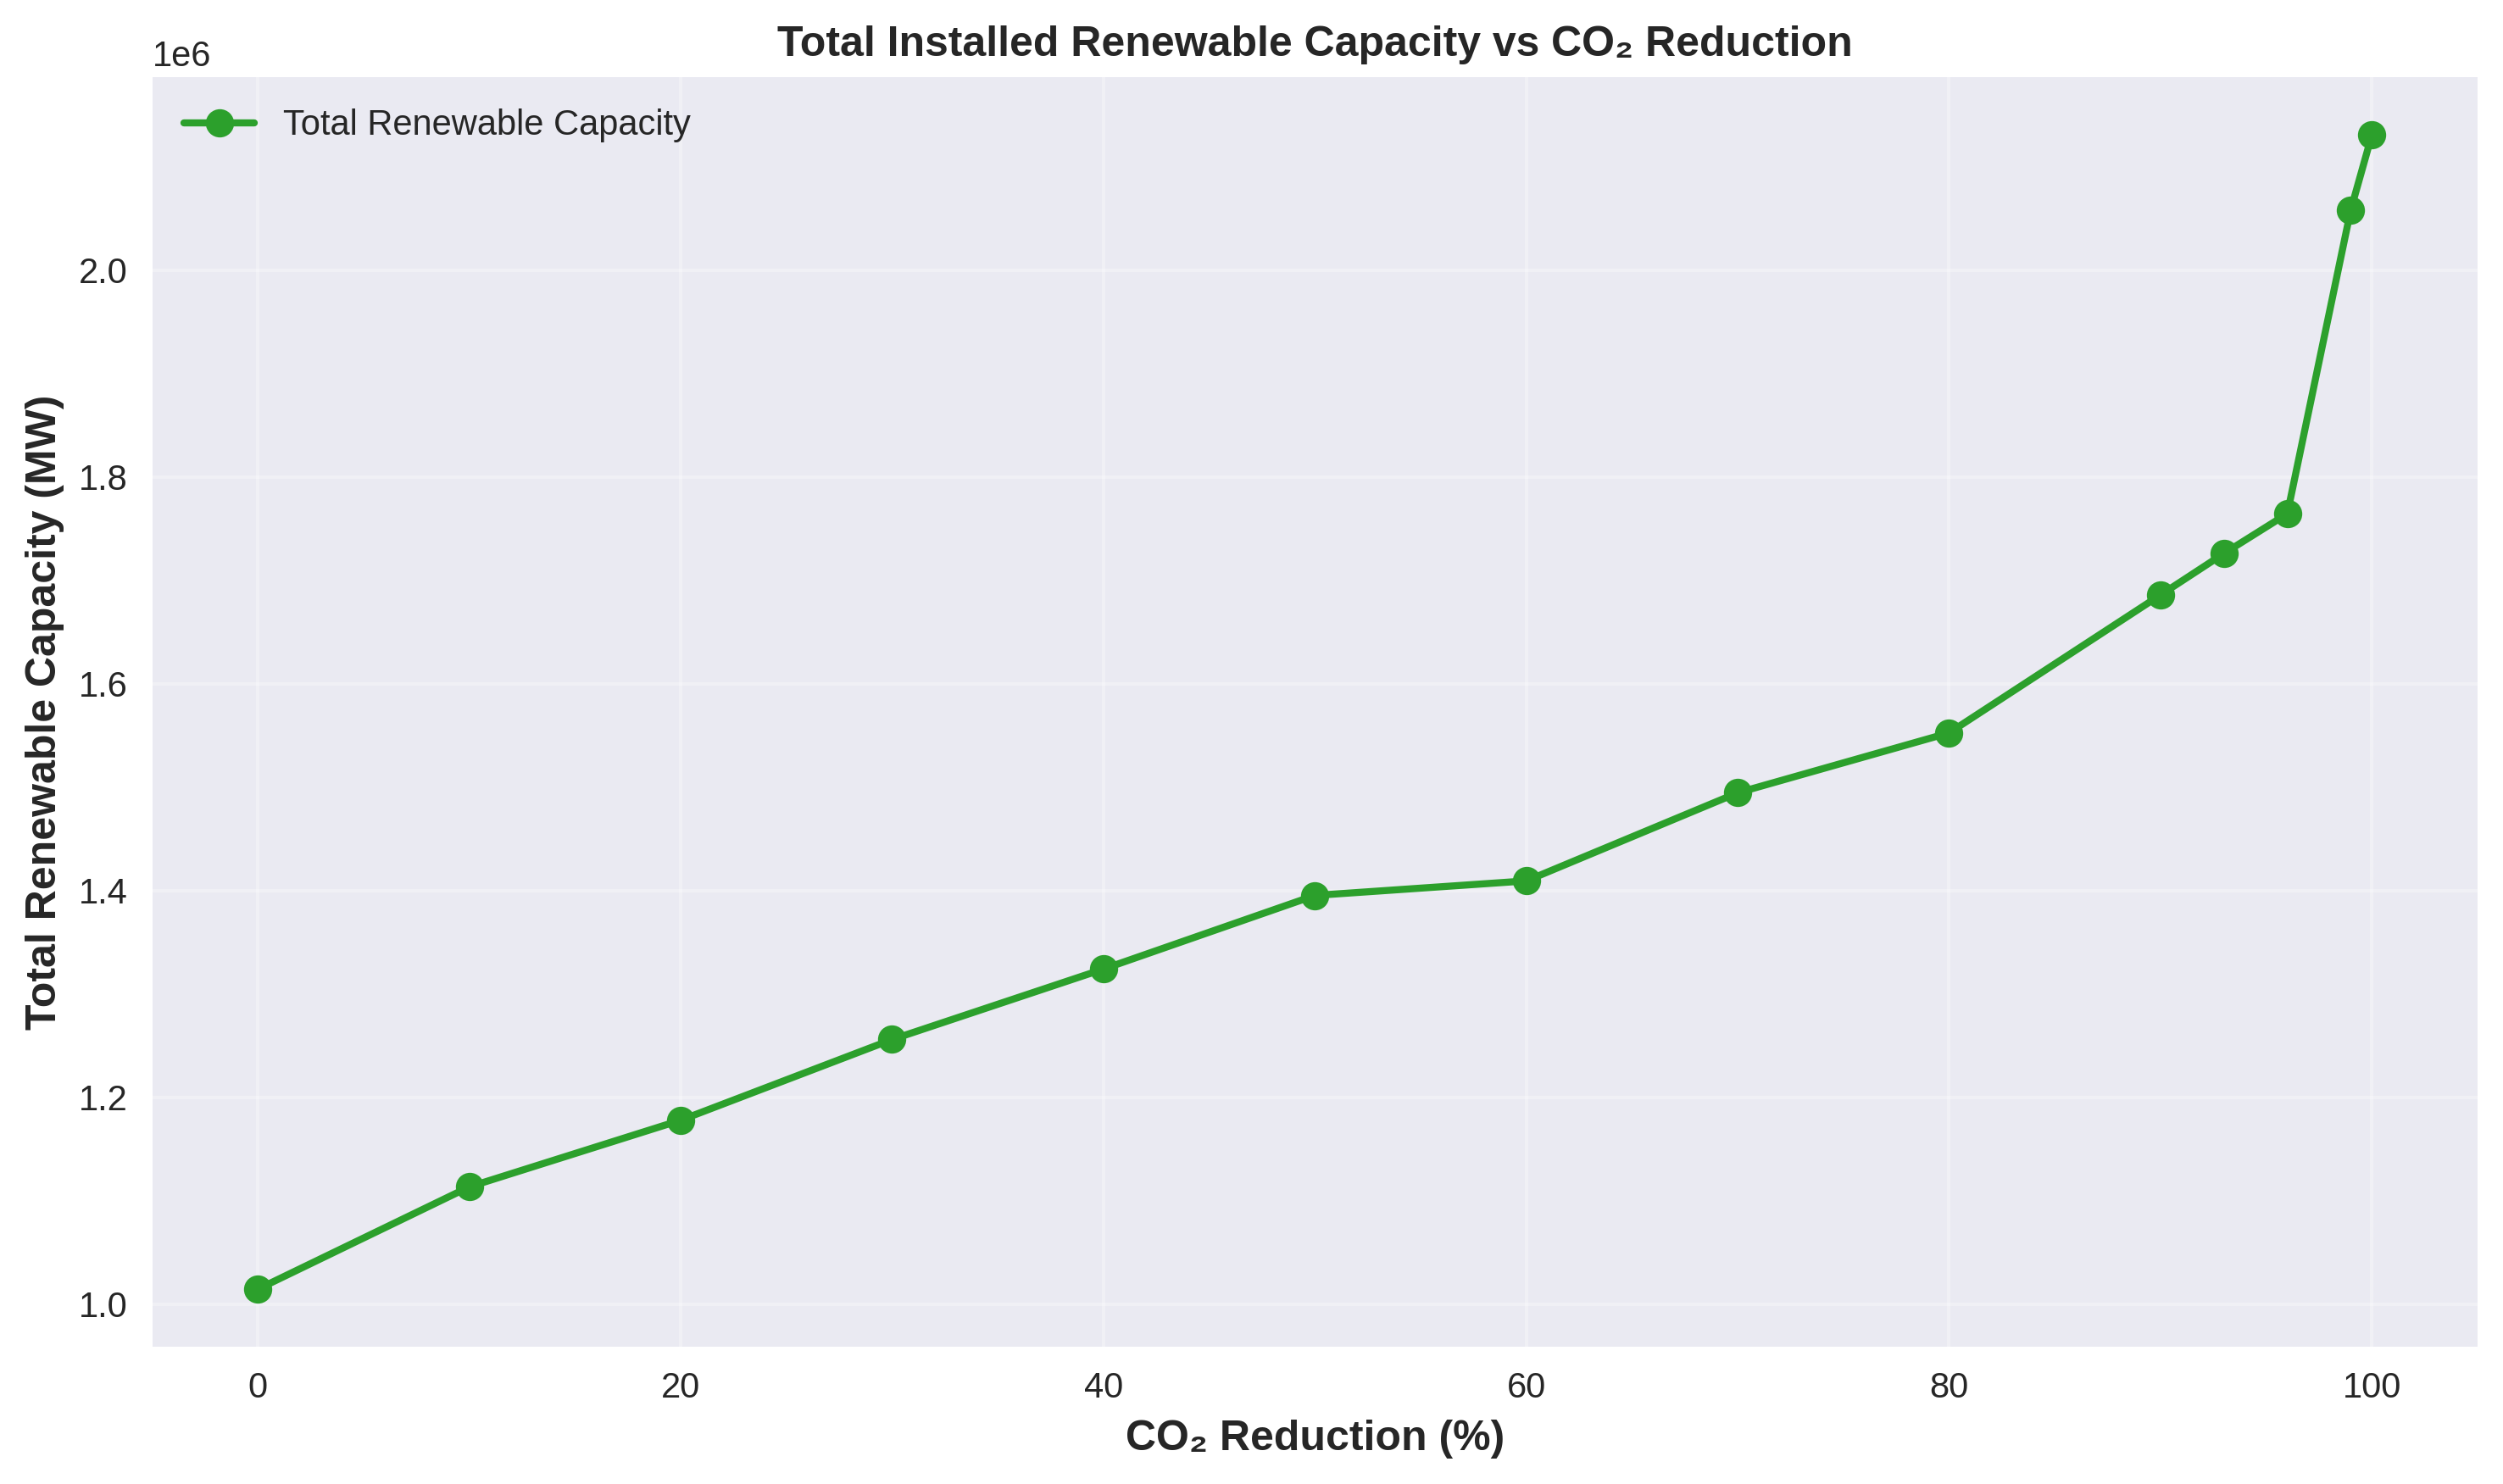
\includegraphics[width=\linewidth]{doc/RenewableCapacity_K_infs.png}
\caption{Figure text}
\label{fig17}
\end{figure}


\medskip
\noindent
\begin{figure}[H]
\centering
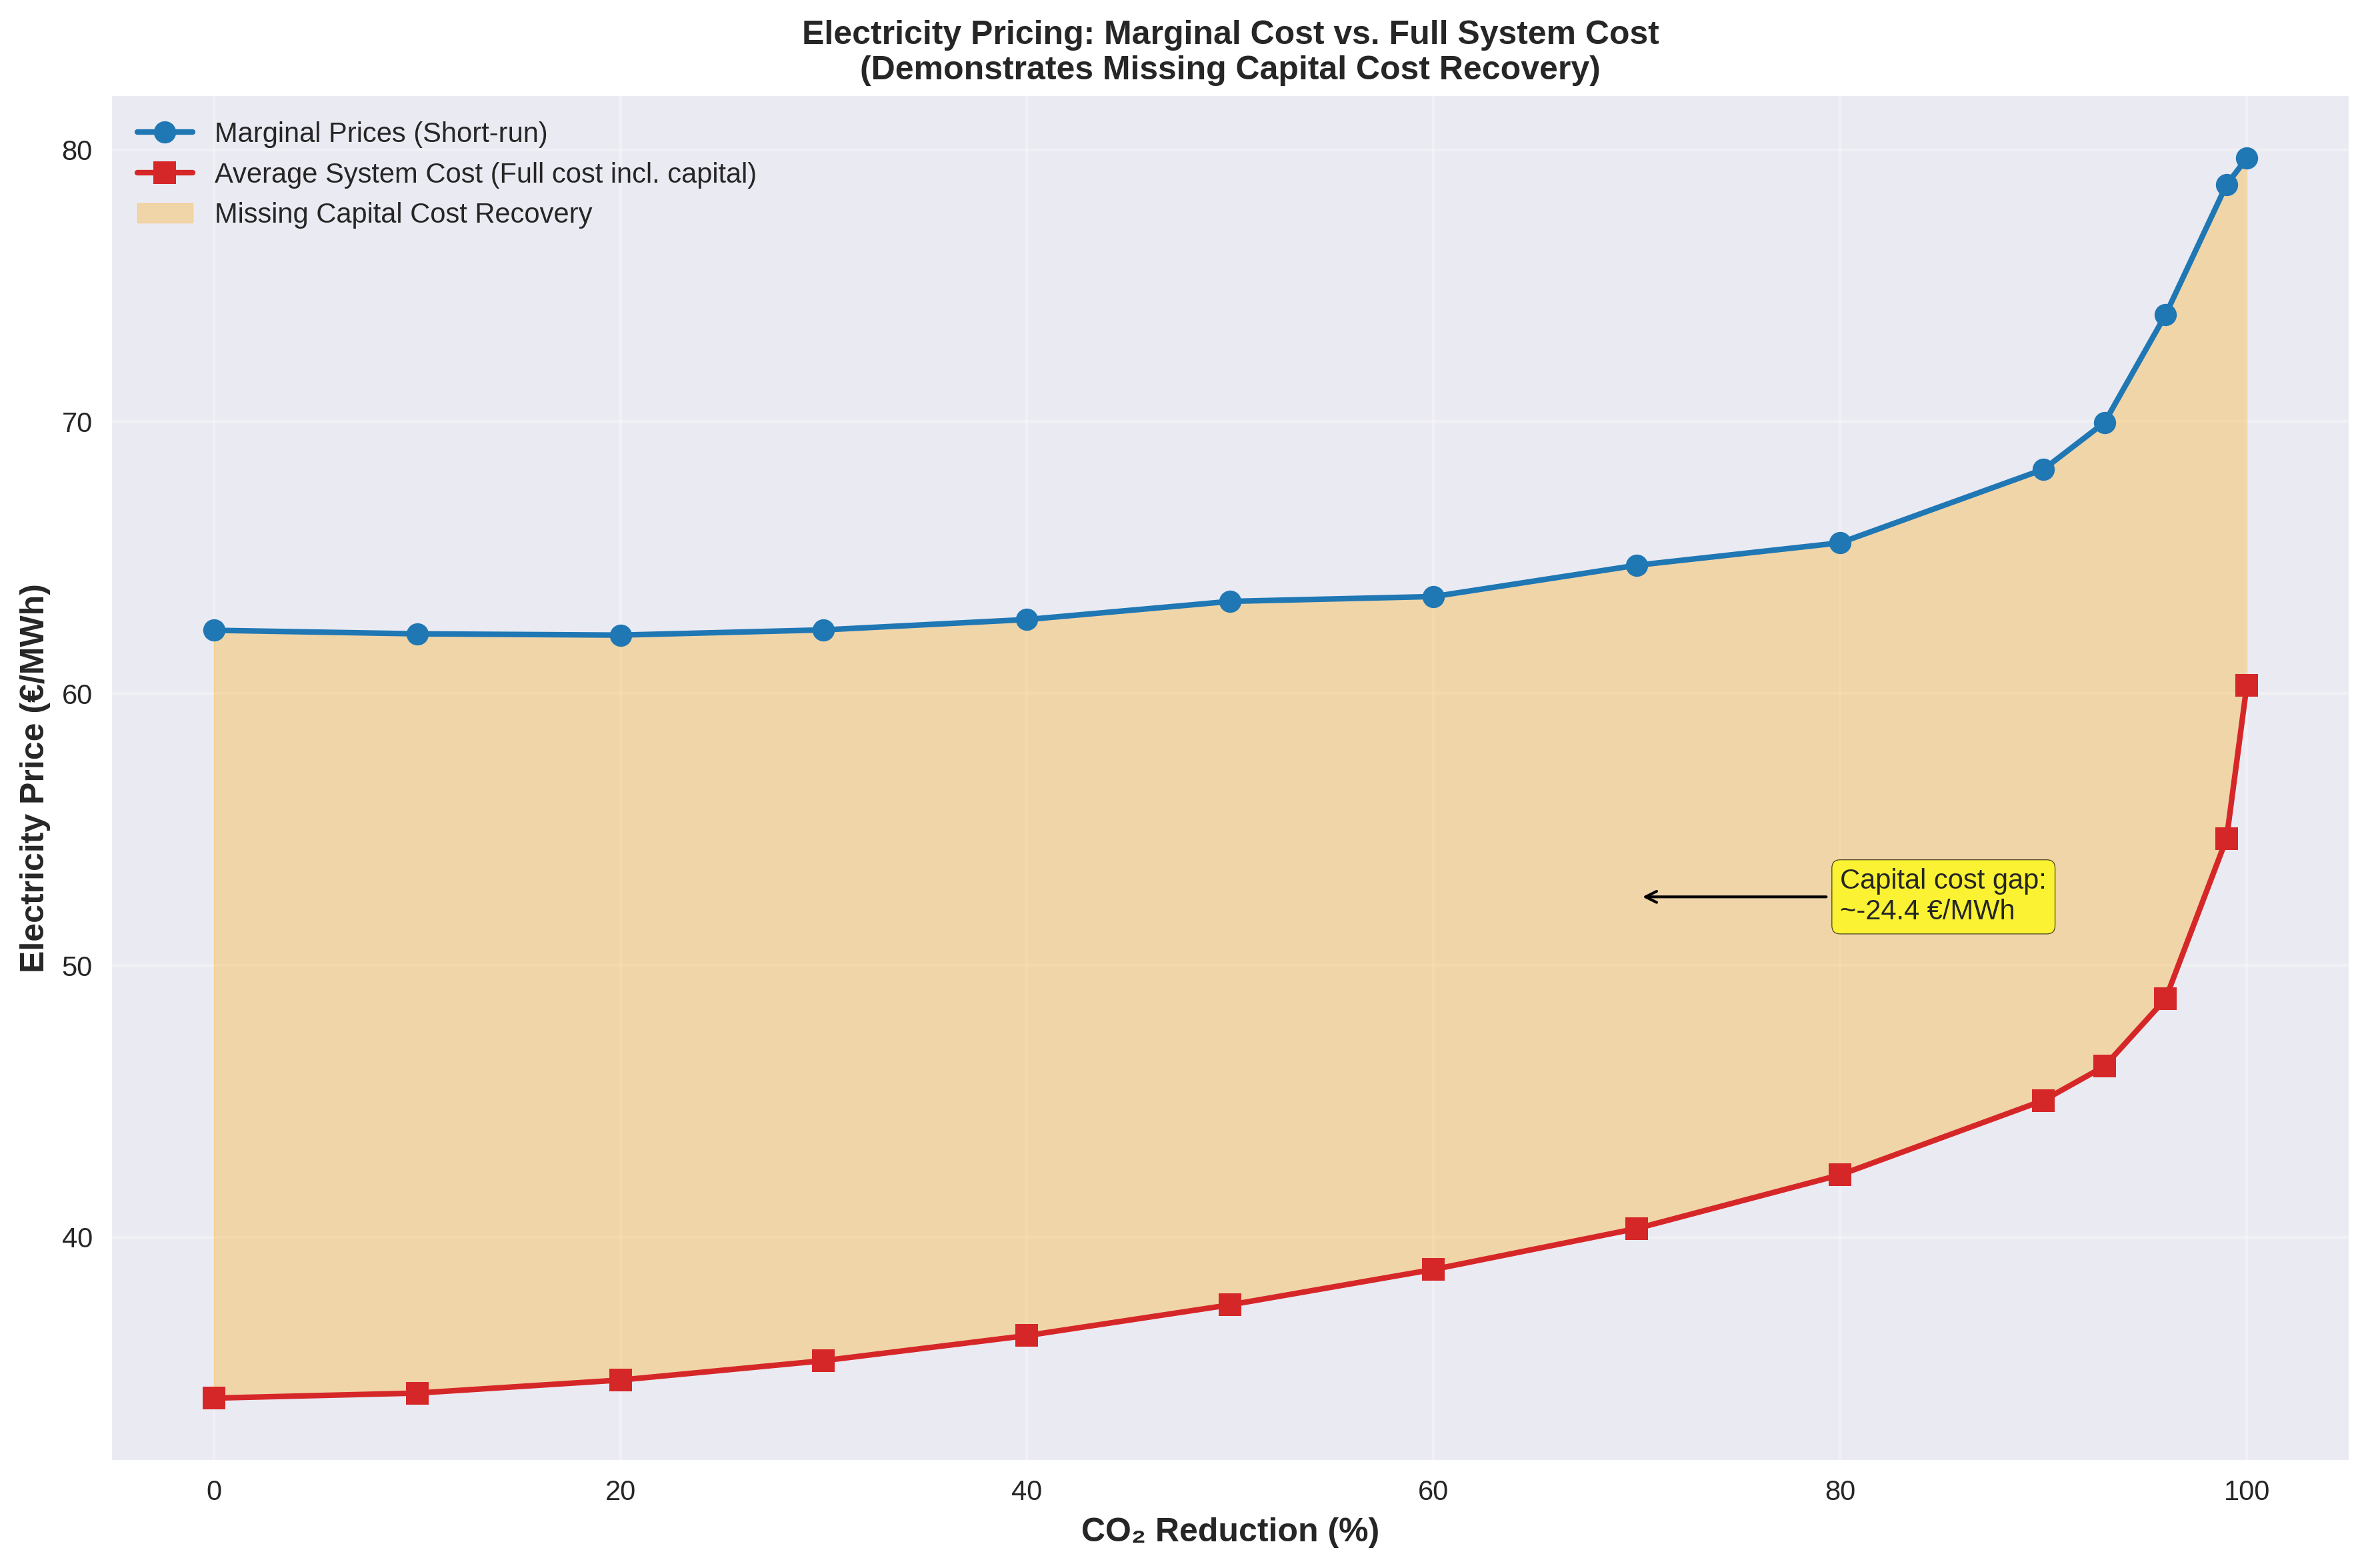
\includegraphics[width=\linewidth]{doc/ElectricityPrices_K_infs.png}
\caption{Figure text}
\label{fig19}
\end{figure}

\medskip
\noindent
\begin{figure}[H]
\centering
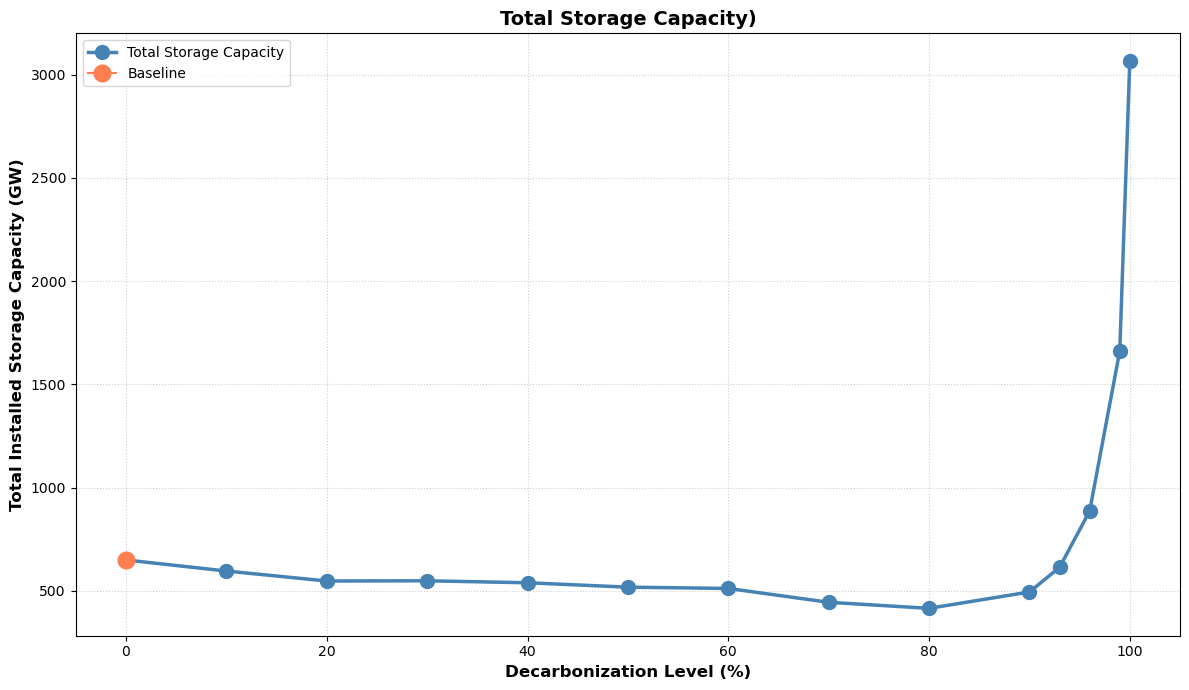
\includegraphics[width=\linewidth]{doc/StorageCapacityMap_K_infs.png}
\caption{Figure text}
\label{fig20}
\end{figure}

\subsubsection{Driving Mechanisms in decarbonizing systems}
Discussing driving mechanisms behind trends like load-following and resource optimization
\subsection{Decentralizing systems}
Introduction to the decentralizing systems showing a few networks and comparing their topology in contrast to their baselines.
\subsubsection{Sanity checks and validations}
Comparing the key figures like marginal prices to those from real networks
\subsubsection{Decentralization trends}
Analyzing how decentralization, de-carbonization and key figures interact. Plotting 3-d response surfaces and discussing shape of solution spaces.
\subsubsection{Driving Mechanisms in decentralizing systems}
Talking about mechanisms that produce the interactions seen above

\section{Discussion}
Introduction to discussion
\subsection{Economic trends and societal paradigms}
What can interactions can be taken from my results and how does this align with expectations and real-world trends
\subsection{Future policy implications}
Discussing how this workflow can be used to analyze and incorporate paradigms to review implications of energy policy.
\subsection{Uses for methodology}
How else could this approach be used and how would this expand the workflows use-case.



\section{Conclusion}

\section{Assumptions}

\section{Acknowledgments}

\section{References}

%% If you have bib database file and want bibtex to generate the
%% bibitems, please use
%%
%%  \bibliographystyle{elsarticle-num} 
%%  \bibliography{<your bibdatabase>}
\bibliographystyle{elsarticle-num}
\bibliography{Sources}

%% Refer following link for more details about bibliography and citations.
%% https://en.wikibooks.org/wiki/LaTeX/Bibliography_Management

\section{Appendices}

Cross reference: \eqref{eq:cost_min}

\medskip
\noindent Inline equation: $CO_{2}$

\noindent Figure reference and figure: \ref{fig1}:



\medskip
\noindent List:
\begin{itemize}
    \item \(S\) represents the set of snapshots,
    \item \(G_r\) is the set of generators located in region \(r\),
    \item \(p_{g,s}\) is the power output of generator \(g\) at snapshot \(s\),
    \item \(e_g\) is the emission factor of generator \(g\), and
    \item \(w_s\) is the weighting factor for snapshot \(s\).
\end{itemize}

\newpage



\end{document}

\endinput
%%
%% End of file `elsarticle-template-num.tex'.
